%
%   $Id$
%   This file is part of the FPC documentation.
%   Copyright (C) 2000 by Florian Klaempfl
%
%   The FPC documentation is free text; you can redistribute it and/or
%   modify it under the terms of the GNU Library General Public License as
%   published by the Free Software Foundation; either version 2 of the
%   License, or (at your option) any later version.
%
%   The FPC Documentation is distributed in the hope that it will be useful,
%   but WITHOUT ANY WARRANTY; without even the implied warranty of
%   MERCHANTABILITY or FITNESS FOR A PARTICULAR PURPOSE.  See the GNU
%   Library General Public License for more details.
%
%   You should have received a copy of the GNU Library General Public
%   License along with the FPC documentation; see the file COPYING.LIB.  If not,
%   write to the Free Software Foundation, Inc., 59 Temple Place - Suite 330,
%   Boston, MA 02111-1307, USA.
%
%%%%%%%%%%%%%%%%%%%%%%%%%%%%%%%%%%%%%%%%%%%%%%%%%%%%%%%%%%%%%%%%%%%%%
% The IDE
%%%%%%%%%%%%%%%%%%%%%%%%%%%%%%%%%%%%%%%%%%%%%%%%%%%%%%%%%%%%%%%%%%%%%
\chapter{The IDE}

The IDE (\textbf{I}ntegrated \textbf{D}evelopment \textbf{E}nvironment)
provides a comfortable user interface to the compiler. It contains an 
editor with syntax highlighting, a debugger, symbol browser etc. 
The IDE is a text-mode application which has the same look and feel 
on all supported operating systems. It is modelled after the IDE of Turbo
Pascal, so many people should feel comfortable using it.

Currently, the IDE is available for \dos, \windows and \linux.

%%%%%%%%%%%%%%%%%%%%%%%%%%%%%%%%%%%%%%%%%%%%%%%%%%%%%%%%%%%%%%%%%%%%%%%
% First steps with the IDE
\section{First steps with the IDE}
%
% Starting the IDE
%
\subsection{Starting the IDE}
The IDE is started by entering the command:
\begin{verbatim}
fp
\end{verbatim}
at the command line. It can also be started from a graphical user 
interface such as \windows. 
\begin{remark}
Under \windows, it is possible to switch between windowed mode and 
full screen mode by pressing \key{Alt-Enter}).
\end{remark}
%
% IDE command-line options.
%
\subsection{IDE Command line options}
When starting the IDE, command line options can be passed:
\begin{verbatim}
fp [-option] [-option] ... <file name> ...
\end{verbatim}
\var{Option} is one of the following switches (the option letters
are case insensitive):
\begin{description}
\item [-N] (\dos only) Do not use long file names. \windows 95 and later
versions of \windows provide an interface to DOS applications to access 
long file names. 
The IDE uses this interface by default to access files. Under certain 
circumstances, this can lead to problems. This switch tells the IDE not to
use the long filenames.
\item [-Cfilename] This option, followed by a filename, tells the IDE to
read its options from \file{filename}. There should be no whitespace between
the file name and the \var{-C}.
\item [-F] use alternative graphic characters. This can be used to run the
IDE on \linux in an X-term or through a telnet session.
\item [-R] After starting the IDE, it changes automatically to the directory
which was active when the IDE exited the last time.
\item [-S] Disable the mouse. When this option is used, then the mouse is
disabled, even if a mouse is present.
\end{description}
The files given at the command line are loaded into edit windows automatically.

\begin{remark}
Under DOS/Win32, the first character of a command-line option can be a \var{/}
character instead of a \var{-} character. So \var{/S} is equivalent to \var{-S}.
\end{remark}

\subsection{The IDE screen}

After start up, the screen of the IDE can look like 
\begin{htmlonly}
this:
\fpcaddimg{../pics/idestart.png}
\end{htmlonly}
\begin{latexonly}
\seefig{idestart}.
\begin{figure}
\caption{The IDE screen immediately after startup}
\label{fig:idestart}
\ifpdf
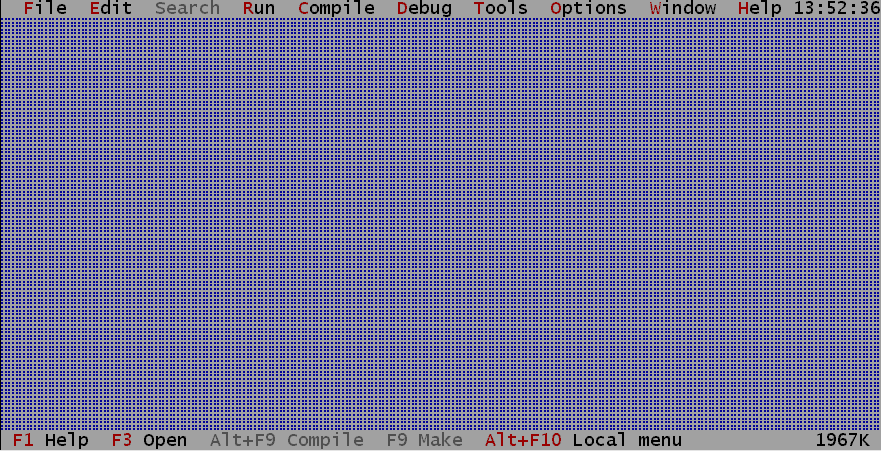
\epsfig{file=pics/idestart.png,width=\textwidth}
\else
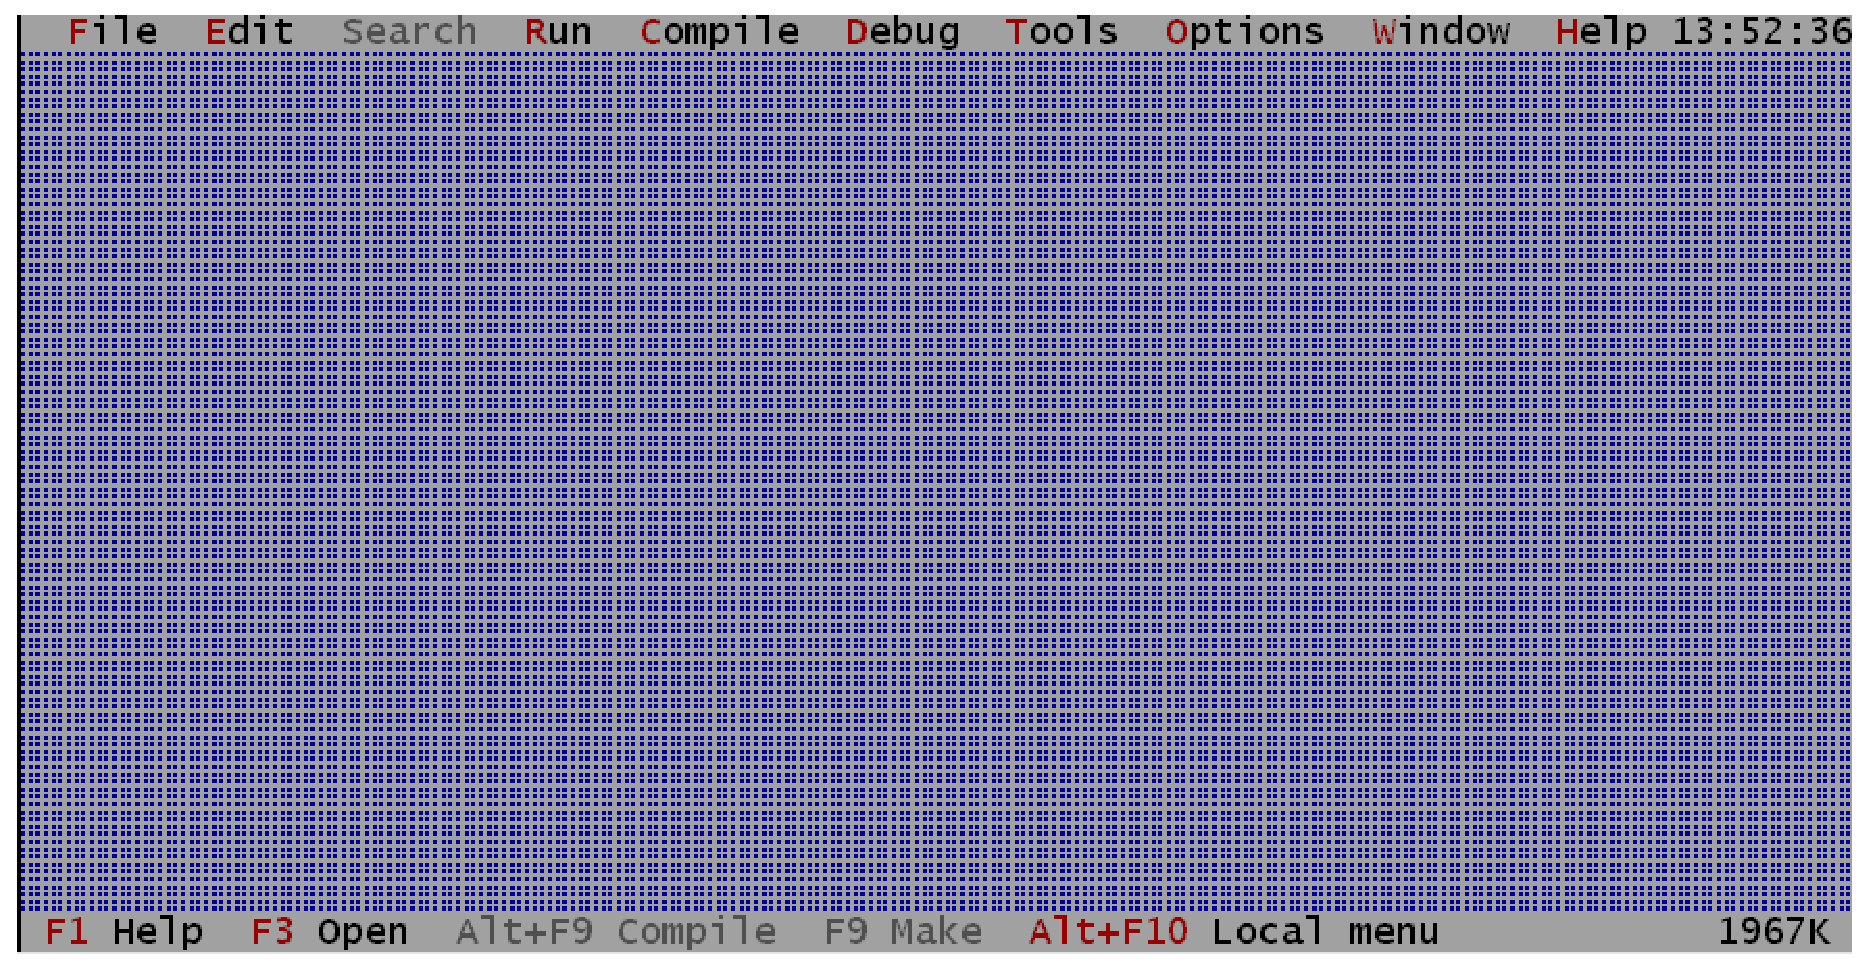
\epsfig{file=pics/idestart.eps,width=\textwidth}
\fi
\end{figure}
\end{latexonly}
At top of the screen the \emph{menu bar} is visible, at the bottom
the \emph{status bar}. The empty space between them is called the
\emph{desktop}.

The status bar shows the keyboard shortcuts for frequently used 
commands, and allows quick access to these commands by clicking 
them with the mouse. 
At the right edge of the status bar, the current amount of unused 
memory is displayed. This is only an indication, since the IDE 
tries to allocate more memory from the operating system if it 
runs out of memory.

The menu provides access to all of the IDE's functionality, and
at the right edge of the menu, a clock is displayed.

The IDE can be left by selecting \menu{File|Exit} in the menu
\footnote{\menu{File|Exit} means select the item 'Exit' in the menu 'File'.}
or by pressing \key{Alt-X}.

\begin{remark}
If a file \file{fp.ans} is found in the current directory,
then it is loaded and used to paint the background.
This file should contain ANSI drawing commands to draw on a screen.
\end{remark}

%%%%%%%%%%%%%%%%%%%%%%%%%%%%%%%%%%%%%%%%%%%%%%%%%%%%%%%%%%%%%%%%%%%%%%%
% Navigating in the IDE
\section{Navigating in the IDE}
The IDE can be navigated both with the keyboard and with a mouse, if the
system is equipped with a mouse.
%
% Using the keyboard
%
\subsection{Using the keyboard} 
All functionality of the IDE is available through use of the keyboard.
\begin{itemize}
\item It is used for typing and navigating through the sources.
\item Editing commands such as copying and pasting text.
\item Moving and resizing windows.
\item It can be used to access the menu, by pressing \key{ALT} and the
appropriate highlighted menu letter, or by pressing \key{F10} and
navigating through the menu with the arrow keys.

more information on the menu can be found in \sees{idemenu}
\item Many commands in the IDE are bound to shortcuts, i.e. typing a special
combination of keys will execute a command immediately.
\end{itemize}
\begin{remark}
\begin{itemize}
\item When working in a \linux X-Term or through a telnet session, the
key combination with \key{Alt} may not be available. To remedy this, the 
\key{Ctrl-Z} combination can be typed first. This means that e.g. \key{Alt-X}
can be replaced by \key{Ctrl-Z X}.
\item A complete reference of all keyboard shortcuts can be found in
\sees{keyshortcuts}.
\end{itemize}
\end{remark}
% 
% Using the mouse
%
\subsection{Using the mouse}
\label{suse:mouseusage}
If the system is equipped with a mouse, it can be used to work with the
IDE. The left button is used to select menu items, press buttons, select
text blocks etc. 

The right mouse button is used to access the local menu, if available.
Holding down the \key{Ctrl} or \key{Alt} key and clicking the right
button will execute user defined functions,  see \sees{prefmouse}.

\begin{remark}
\begin{enumerate}
\item Occasionally, the manual uses the term "drag the mouse". This
means that the mouse is moved while the left mouse button is being 
pressed.
\item 
The action of mouse buttons may be reversed, i.e. the actions of the left
mouse button can be assigned to the right mouse button and vice versa  
\footnote{See \sees{prefmouse} for more information on how to reverse the
actions of the mouse buttons.}. Throughout the manual, it is assumed 
that the actions of the mouse buttons are not reversed.
\item
The mouse is not always available, even if a mouse is installed:
\begin{itemize}
\item The IDE is running under \linux through a telnet connection from 
a \windows machine.
\item The IDE is running under \linux in an X-term under X-windows.
\end{itemize}
\end{enumerate}
\end{remark}
%
% Navigating in dialogs
% 
\subsection{Navigating in dialogs}
\label{se:navigatingdialogs}
Dialogs usually have a lot of elements in them such as buttons, edit fields,
memo fields, list boxes and so on. To activate one of these fields, it is
sufficient to:
\begin{enumerate}
\item Click on the element with the mouse.
\item Press the \key{Tab} key till the focus reaches the mouse
\item Press the highlighted letter in the element's label. If the focus
is currently on an element that allows to edit, then \key{Alt} should be
pressed simultaneously with the highlighted letter. For a button, the action
associated with the button will then be executed.
\end{enumerate}
Inside edit fields, list boxes, memos, navigation is carried out with the
usual arrow key commands.

%%%%%%%%%%%%%%%%%%%%%%%%%%%%%%%%%%%%%%%%%%%%%%%%%%%%%%%%%%%%%%%%%%%%%%%
% Windows
\section{Windows}
\label{se:windows}
Nowadays, working with windowed applications should be no problem for
most \windows and \linux users. Nevertheless, the following section 
describes how the windows work in the \fpc IDE, to allow efficient 
work with it.
%
% Window basics
%
\subsection{Window basics}
\label{se:windowbasics}
\begin{htmlonly}
A common IDE window is displayed  below:
\fpcaddimg{../pics/idewin.png}
\end{htmlonly}
\begin{latexonly}
A common IDE window is displayed in \seefig{idewin}.
\begin{figure}
\caption{A common IDE window}
\label{fig:idewin}
\ifpdf
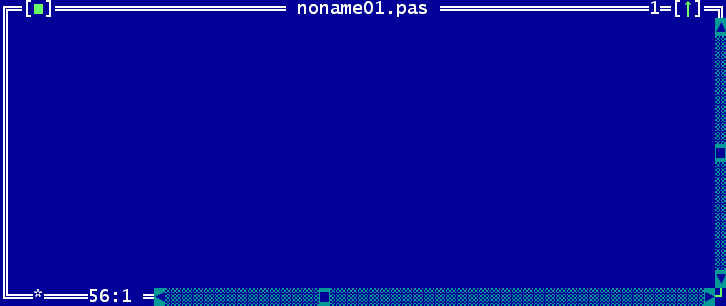
\epsfig{file=pics/idewin.png,width=\textwidth}
\else
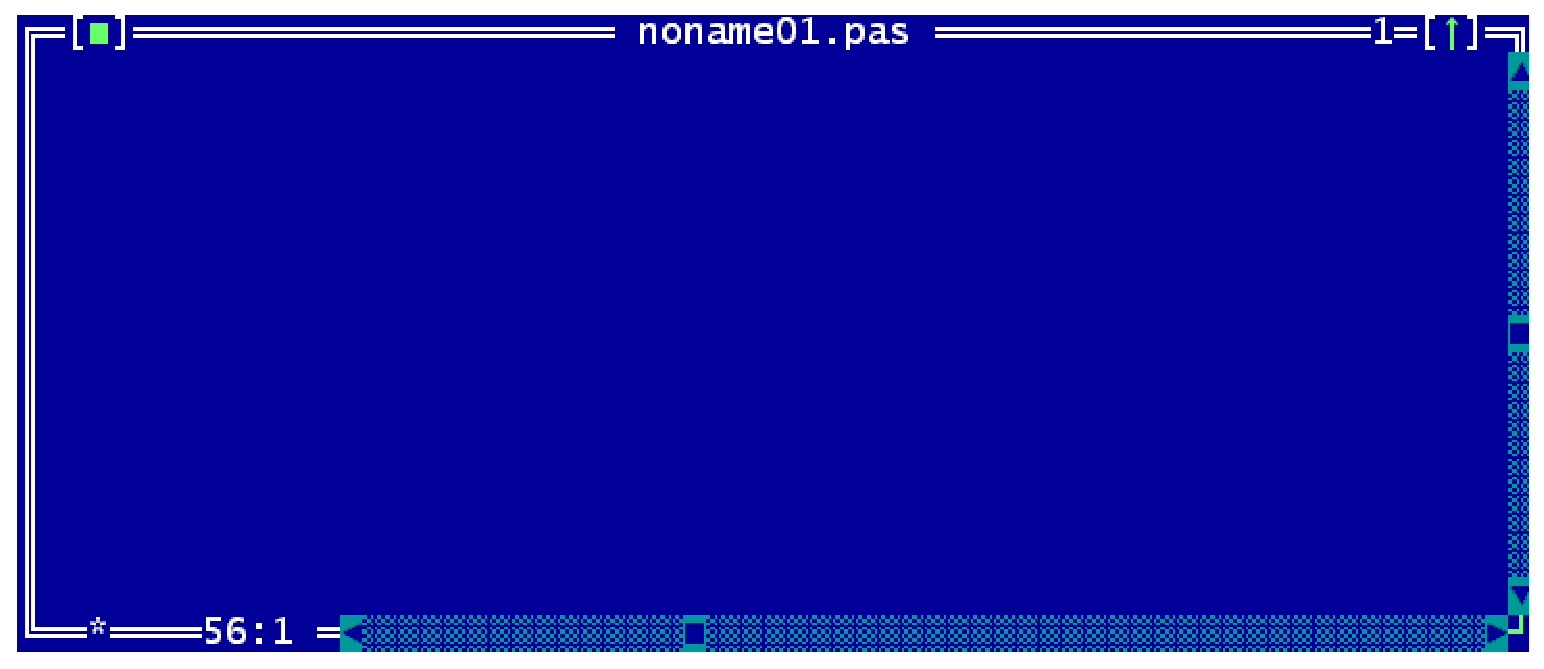
\epsfig{file=pics/idewin.eps,width=\textwidth}
\fi
\end{figure}
\end{latexonly}
The window is surrounded by a so-called \emph{frame}, the white double
line around the window. 

At the top of the window 4 things are displayed:
\begin{itemize}
\item 
At the upper left corner of the window, a \emph{close icon} is shown. 
When clicked, the window will be closed. It can be also closed by
 pressing \key{Alt-F3} or selecting the menu item \menu{Window|Close}. 
All open windows can be closed by selecting the menu item 
\menu{Window|Close all}.
\item In the middle, the title of the window is displayed.
\item Almost at the upper right corner, a number is visible.
This number identifies the editor window, and pressing \key{Alt-Number}
will jump to this window. Only the first 9 windows will get such a number.
\item At the upper right corner, a small green arrow is visible.
Clicking this arrow zooms the window so it covers the whole desktop. 
Clicking this arrow on a zoomed window will restore old size of the 
window. Pressing the key \key{F5} has the same effect as clicking 
that arrow. The same effect can be achieved with the menu item 
\menu{Window|Zoom}. 
Windows and dialogs which aren't resizeable can't be zoomed, either.
\end{itemize}

The right edge and bottom edges of a window contain scrollbars.
They can be used to scroll the window contents with the mouse. 
The arrows at the ends of the scrollbars can be clicked to scroll the 
contents line by line. Clicking on the dotted area between the arrows 
and the cyan-coloured rectangle will scroll the window's content 
page by page. By dragging the rectangle the content can be scrolled 
continuously.

The star and the numbers in the lower left corner of the window
display information about the contents of the window. They
are explained in the section about the editor, see \sees{editingtext}.

%
% Sizing+moving windows
%
\subsection{Sizing and moving windows}
\label{se:windowsizingmoving}
A window can be moved and sized using the mouse and the keyboard:
To move a window:
\begin{itemize}
\item using the mouse, click on the title bar and drag the window 
with the mouse.
\item using the keyboard, go into the size/move mode
by pressing \key{Ctrl-F5} or selecting the menu item
\menu{Window|Size/Move}. . Using the cursor keys the window can be moved. 
The size/move mode can be left by pressing \key{Enter}. 
In this case, the window will keep its size and position. 
Alternatively, pressing \key{Esc} will restore the old position.
\end{itemize} 
To resize a window:
\begin{itemize}
\item using the mouse, click on the lower right corner of the window
and drag it.
\item using the keyboard, go into the size/move mode
by pressing \key{Ctrl-F5} or selecting the menu item
\menu{Window|Size/Move}. The window frame will be green to indicate that
the IDE is in size/move mode. 
By pressing shift and the cursor keys simultaneously, the window can 
be resized.  The size/move mode can be left by pressing
\key{Enter}. In this case, the window will keep the new size.
Pressing \key{Esc} will restore the old size.
\end{itemize}
Not all windows can be resized. This applies, for example, to
\emph{dialog windows} (\sees{dialogwindow}).

A window can also be hidden. To hide a window, the \key{Ctrl-F6} key
combination can be used, or the \menu{Window|Hide} menu may be selected.
To restore a Hidden window, it is necessary to select it from the window
list. More information about the window list can be found in the next
section.   
%
% Multiple windows
%
\subsection{Working with multiple windows}
\label{se:multiplewindows}
When working with larger projects, it is likely that multiple windows 
will appear on the desktop. However, only one of these windows will be 
the active window, all other windows will be inactive.

An inactive window is identified by a grey frame. An inactive window can
be made active in one of several ways:
\begin{itemize}
\item using the mouse, activate a window by clicking on it.
\item using the keyboard, pressing \key{F6} will step trough all open 
windows. To activate the previously activated window, \key{Shift-F6} can
be used.
\item the menu item \menu{Window|Next} can be used to activate the next 
window in the list of windows, while \var{Window|Previous} will select
the previous window.
\item If the window has a number in the upper right corner, it can be
activated by pressing \key{Alt-<number>}.
\item Pressing \key{Alt-0} will pop up a dialog with all 
available windows which allows a quick activation of windows which 
don't have a number.
\end{itemize}

The windows can be ordered and placed on the IDE desktop by zooming and
resizing them with the mouse or keyboard. This is a time-consuming task, 
and particularly difficult with the keyboard. Instead, the menu items
\menu{Window|Tile} and \menu{Window|Cascade} can be used:
\begin{description}
\item[Tile] will divide whole desktop space evenly between all resizable 
windows. 
\item[Cascade] puts all windows in a cascaded position. 
\end{description}

In very rare cases the screen of the IDE may be mixed up. In this
case the whole IDE screen can be refreshed by selecting the menu item 
\menu{Window|Refresh display}.
%
% Dialog windows
%
\subsection{Dialog windows}
\label{se:dialogwindow}
In many cases the IDE displays a dialog window to get user input.
The main difference to normal windows is that other windows cannot be
activated while a dialog is active. Also the menu is not accessible while in
a dialog. This behaviour is called \emph{modal}. To activate another window, 
the modal window or dialog must be closed first.

\begin{htmlonly}
A typical dialog window looks like:
\fpcaddimg{../pics/idedlg.png}
\end{htmlonly}
\begin{latexonly}
A typical dialog window is shown in \seefig{idedlg}.
\begin{figure}
\caption{A typical dialog window}
\label{fig:idedlg}
\ifpdf
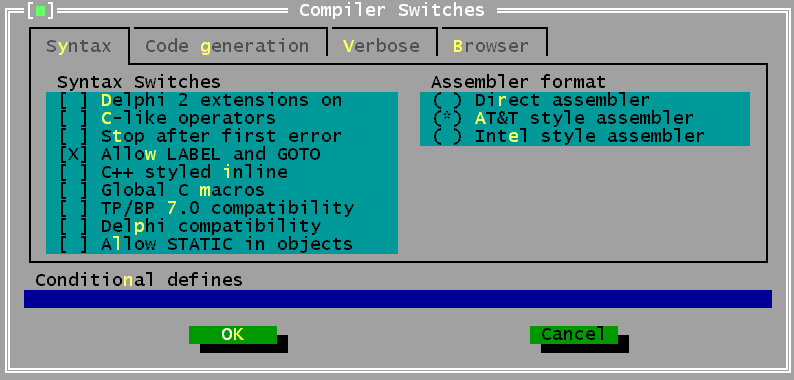
\epsfig{file=pics/idedlg.png,width=\textwidth}
\else
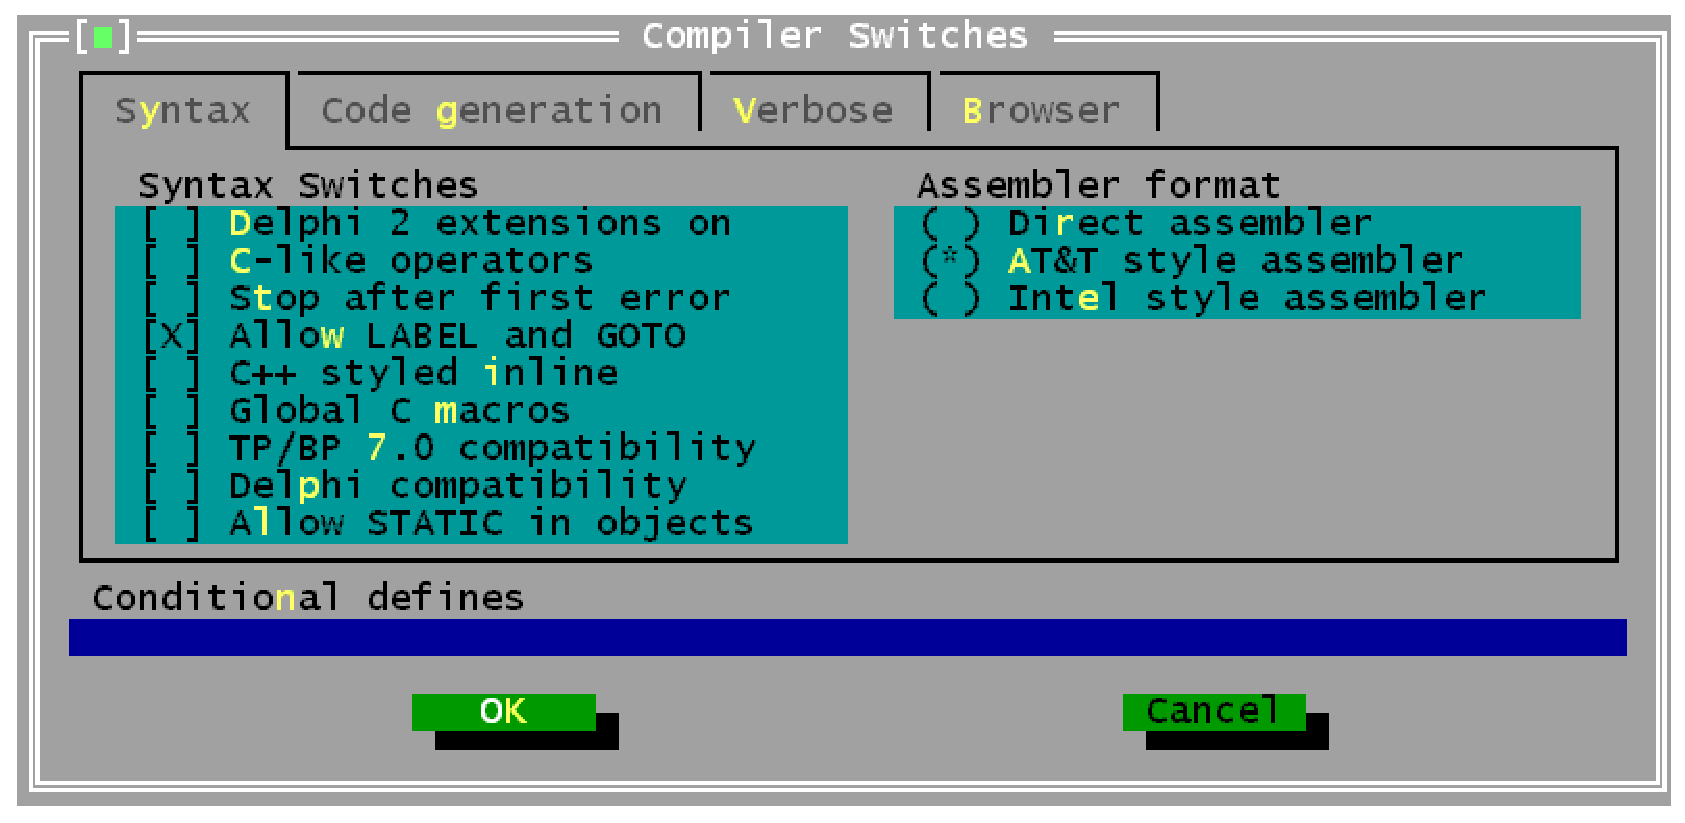
\epsfig{file=pics/idedlg.eps,width=\textwidth}
\fi
\end{figure}
\end{latexonly}

%%%%%%%%%%%%%%%%%%%%%%%%%%%%%%%%%%%%%%%%%%%%%%%%%%%%%%%%%%%%%%%%%%%%%%%
% The menu
\section{The Menu}
\label{se:idemenu}
The main menu (the gray bar at the top of the IDE) provides access to all the
functionality of the IDE. It also displays a clock, displaying the current
time. The menu is always available, except when a dialog is opened. If a
dialog is opened, it must be closed first in order to access the menu.

In certain windows, a local menu is also available. The local menu will
appear where the cursor is, and provides additional commands that are 
context-sensitive.
%
% Accessing the menu
%
\subsection{Accessing the menu}
The menu can be accessed in a number of ways:
\begin{enumerate}
\item By using the mouse to select items. The mouse cursor should be located
over the desired menu item, and a left mouse click will then select it.
\item By pressing \key{F10}. This will switch the IDE focus to the menu. 
Use the arrow keys can then be used to navigate in the menu, the 
\key{Enter} key should be used to select items.
\item To access menu items directly, \key{Alt-<highlighted menu letter>}
can be used to select a menu item. Afterwards submenu entries can be selected 
by pressing the highlighted letter, but without \key{Alt}. 
E.g. \key{Alt-S G} is a fast way to display the \emph{goto line} dialog.
\end{enumerate}
Every menu item is explained by a short text in the status bar.

When a local menu is available, it can be accessed by pressing
the right mouse button or \key{Alt-F10}. 

In the subsequent, all menu entries and their actions are described.
%
% The file menu
%
\subsection{The File menu}
\label{se:menufile}
The \menu{File} menu contains all menu items that allow to load and save
files, as well as to exit the IDE.
\begin{description}
\item[New] Opens a new, empty editor window. 
\item[New from template] Prompts for a template to be used, asks to fill in
any parameters, and then starts a new editor window with the template.
\item[Open] (\key{F3}) Presents a file selection dialog, and opens 
the selected file in a new editor window. 
\item[Save] (\key{F2}) Saves the contents of the current edit window 
with the current filename. If the current edit window does not yet have
a filename, a dialog is presented to enter a filename.
\item[Save as] Presents a dialog in which a filename can be entered. The
current window's contents are then saved to this new filename, and the
filename is stored for further save actions.
\item[Change dir] Presents a dialog in which a directory can be selected.
The current working directory is then changed to the selected directory.
\item[Command shell] Executes a command shell. After the shell exited, the
IDE resumes. Which command shell is executed depends on the system. 
\item[Exit] (\key{ALT-X}) Exits the IDE. If any unsaved files are 
in the editor, the IDE will ask if these files should be saved.
\end{description}
Under the \menu{Exit} menu appear some filenames of recently used files.
These entries can be used to quickly reload these files in the editor.

%
% The edit menu
%
\subsection{The Edit menu}
\label{se:menuedit}
The \menu{Edit} menu contains entries for accessing the clipboard, and
undoing or redoing editing actions. Most of these functions have shortcut
keys associated with them.
\begin{description}
\item[Undo] (\key{ALT-BKSP})
Undo the last editing action. The editing actions are stored in a buffer,
selecting this mechanism will move backwards through this buffer, i.e.
multiple undo levels are possible. The selection is not preserved, though.
\item[Redo] Redo the last action that was previously undone. Redo can redo
multiple undone actions. 
%\item[Dump undo]
%Shows the contents of the UNDO list in the messages window.
%\item[Undo all]
%Undo all actions in the undo buffer. If a new empty file was started, this
%action should clear the window contents again.
%\item[Redo all]
%Redo all editing actions that were undone.
\item[Cut] (\key{Shift-DEL}) Copy the current selection to the clipboard
and delete the selection from the text. Any previous clipboard contents is
lost after this action. After this action, the clipboard contents can be 
pasted elsewhere in the text.
\item[Copy] (\key{Ctrl-INS}) Copy the current selection to the clipboard.
Any previous clipboard contents is lost after this action. 
After this action, the clipboard contents can be pasted elsewhere in the text.
\item[Paste] (\key{Shift-INS}) Insert the current clipboard contents in
the text at the cursor position. The clipboard contents remains as it was.
\item[Clear] (\key{Ctrl-DEL}) Clears (i.e. deletes) the current
selection.
\item[Show clipboard] Opens a window in which the current clipboard contents
is shown.
\end{description}
When running an IDE under \windows, the \menu{Edit} menu has two
additional entries. The IDE maintains a separate clipboard which does 
not share its contents with the windows clipboard. To access the Windows
clipboard, the following two entries are also present:
\begin{description}
\item[Copy to Windows] this will copy the selection to the Windows
clipboard. 
\item[Paste from Windows] this will insert the content of the windows
clipboard (if it contains text) in the edit window at the current cursor
position.
\end{description}

%
% The Search menu
%
\subsection{The Search menu}
\label{se:menusearch}
The \menu{Search} menu provides access to the search and replace dialogs, as well as
access to the symbol browser of the IDE. 
\begin{description}
\item[Find] (\key{Ctrl-Q F}) Presents the search dialog. A search text 
can be entered, and when the dialog is closed, the entered text is searched
in the active window. If the text is found, it will be selected. 
\item[Replace] (\key{Ctrl-Q A}) Presents the search and replace dialog.
After the dialog is closed, the search text will be replaced by the replace
text in the active window.
\item[Search again] (\key{CTRL-L}) Repeats the last search or search and replace action,
 using  the same parameters.
\item[Go to line number] (\key{Alt-G}) Prompts for a line number, and
then jumps to this line number.
\end{description}
When the program and units are compiled with browse information, then
the following menu entries are also enabled:
\begin{description}
\item[Find procedure]
Not yet implemented.
\item[Objects]
Asks for the name of an object and opens a browse window for this object.
\item[Modules]
Asks for the name of a module and opens a browse window for this object.
\item[Globals]
Asks for the name of a global symbol and opens a browse window for this object.
\item[Symbol]
Opens a window with all known symbols, so a symbol can be selected. After
the symbol is selected, a browse window for that symbol is opened.
\end{description}
%
% The Run menu
%
\subsection{The Run menu}
\label{se:menurun}
The \menu{Run} menu contains all entries related to running a program,
\begin{description}
\item[Run] (\key{Ctrl-F9})
If the sources were modified, compiles the program. If the compile is
successful, the program is executed. If the primary file  was set, then 
that is used to determine which program to execute. See \sees{menucompile}
for more information on how to set the primary file.
\item[Step over] (\key{F8})
Run the program till the next source line is reached. If any calls to 
procedures are made, these will be executed completely as well.
\item[Trace into] (\key{F7})
Execute the current line. If the current line contains a call to another
procedure, the process will stop at the entry point of the called procedure.
\item[Goto cursor] (\key{F4})
Runs the program till the execution point matches the line where the cursor
is.
\item[Until return]
Runs the current procedure till it exits.
\item[Parameters]
This menu item allows to enter parameters that will be passed on to the
program when it is being executed.
\item[Program reset] (\key{Ctrl-F2}) if the program is being run or 
debugged, the debug session is aborted, and the running program is killed.
\end{description}
%
% The compile menu
%
\subsection{The Compile menu}
\label{se:menucompile}
The \menu{Compile} menu contains all entries related to compiling a program or
unit.
\begin{description}
\item[Compile] (\key{Alt-F9}) Compiles the contents of the active window,
irrespective of the primary file setting.
\item[Make] (\key{F9}) Compiles the contents of the active window, and
any files that the unit or program depends on and that were modified since
the last compile.
If the primary file was set, the primary file is compiled instead.
\item[Build]
Compiles the contents of the active window, and any files that the unit or 
program depends on, whether they were modified or not.
If the primary file was set, the primary file is compiled instead.
\item[Target] Sets the target operating system for which should be compiled. 
\item[Primary file] Sets the primary file. If set, any run or compile command 
will act on the primary file instead of on the active window. The primary
file need not be loaded in the IDE for this to have effect.
\item[Clear primary file]
Clears the primary file. After this command, any run or compile action will
act on the active window.
\item[Information] Displays some information about the current program.
\item[Compiler messages] (\key{F12}) Displays the compiler messages
window. This window will display the messages generated by the compiler
during the last compile.
\end{description}
%
% The debug menu
%
\subsection{The Debug menu}
\label{se:menudebug}
The \menu{Debug} menu contains menu entries to aid in debugging a program, such as
setting breakpoints and watches. 
\begin{description}
\item[Output]
\item[User screen] (\key{Alt-F5})
Switches to the screen as it was last left by the running program.
\item[Breakpoint] (\key{Ctrl-F8})
Sets a breakpoint at the current line. When debugging, program execution
will stop at this breakpoint.
\item[Call stack] (\key{Ctrl-F3})
Shows the call stack. The call stack is the list of addresses (and
filenames and line numbers, if this information was compiled in) of 
procedures that are currently being called by the running program.
\item[Registers]
Shows the current content of the CPU registers. 
\item[Add watch] (\key{Ctrl-F7}) Add a watch. A watch is an expression
that can be evaluated by the IDE and will be shown in a special window. 
Usually this is the content of some variable. 
\item[Watches]
Shows the current list of watches in a separate window.
\item[Breakpoint list]
Shows the current list of breakpoints in a separate window.
\item[GDB window]
Shows the GDB debugger console. This can be used to interact with the debugger
directly; here arbitrary GDB commands can be typed and the result will be
shown in the window.
\end{description}
%
% The tools menu
%
\subsection{The Tools menu}
\label{se:menutools}
The \menu{Tools} menu defines some standard tools. If new tools are defined by the
user, they are appended to this menu as well.
\begin{description}
\item[Messages] (\key{F11}) Show the messages window. 
This window contains the output from one of the tools. For more information,
see \sees{toolsmessages}.
\item[Goto next] (\key{Alt-F8}) Goto next message.
\item[Goto previous] (\key{Alt-F7}) Goto previous message
\item[Grep] (\key{SHIFT-F2}) Prompts for a regular expression and options
to be given to grep, and then executes \file{grep} with the given expression and
options. For this to work, the \file{grep} program must be installed on the
system, and be in a directory that is in the \var{PATH}. For more
information, see \sees{grep}.
\item[Calculator] 
Displays the calculator. For more information, see \sees{calculator}
\item[Ascii table] Displays the \var{ASCII} table. For more information, see
\sees{asciitable}
\end{description}
%
% The Options menu
%
\subsection{The Options menu}
\label{se:menuoptions}
The \menu{Options} menu is the entry point for all dialogs that are used to set
options for compiler and IDE, as well as the user preferences.
\begin{description}
\item[Mode] Presents a dialog to set the current mode of the compiler. The
current mode is shown at the right of the menu entry. For more information,
see \sees{compilermode}.
\item[Compiler] Presents a dialog that can be used to set common compiler
options. These options will be used when compiling a program or unit.
\item[Memory sizes]
Presents a dialog where the stack size and the heap size for the program can
be set. These options will be used when compiling a program.
\item[Linker]
Presents a dialog where some linker options can be set. These options will
be used when a program or library is compiled.
\item[Debugger]
Presents a dialog where the debugging options can be stored. These options
are used when compiling units or programs. Note that the debugger will not
work unless debugging information is generated in the program.
\item[Directories]
Presents a dialog where the various directories needed by the compiler can
be set. These directories will be used when a program or unit is compiled.
\item[Browser]
Presents a dialog where the browser options can be set. The browser options
affect the behaviour of the symbol browser of the IDE. 
\item[Tools]
Presents a dialog to configure the tools menu. For more information, see
\sees{addingtools}.
\item[Environment]
Presents a dialog to configure the behaviour of the IDE. A sub menu is
presented with the various aspects of the IDE:
\begin{description}
\item[Preferences]
General preferences, such as whether to save files or not, and which files
should be saved. The video mode can also be set here.
\item[Editor]
Controls various aspects of the edit windows.
\item[CodeComplete]
Used to set the words which can be automatically completed when typing in
the editor windows.
\item[Codetemplates]
Used to define code templates, which can be inserted in an edit window.
\item[Desktop]
Used to control the behaviour of the desktop, i.e. several features can be
switched on or off.
\item[Mouse]
Can be used to control the actions of the mouse, and to assign commands to
various mouse actions.
\item[Startup]
Not yet implemented.
\item[Colors]
Here the various colors used in the IDE and the editor windows can be set.
\end{description}
\item[Open]
Presents a dialog in which a file with editor preferences can be selected. 
after the dialog is closed, the preferences file will be read and the
preferences will be applied.
\item[Save]
Save the current options in the default file.
\item[Save as]
Saves the current options in an alternate file. A file selection dialog box
will be presented in which the alternate settings file can be entered.
\end{description}
Please note that options are not saved automatically, they should be saved
explicitly with the \menu{Options|\-Save} command.
%
% The window menu
%
\subsection{The Window menu}
\label{se:menuwindow}
The \menu{Window} menu provides access to some window functions. More information
on all these functions can be found in \sees{windows}
\begin{description}
\item[Tile]
Tiles all opened windows on the desktop.
\item[Cascade]
Cascades all opened windows on the desktop.
\item[Close all]
Close all opened windows.
\item[Size/move] (\key{Ctrl-F5})
Put the IDE in Size/move modus; after this command the active window can be
moved and resized using the arrow keys.
\item[Zoom] (\key{F5})
Zooms or unzooms the current window. 
\item[Next] (\key{F6})
Activates the next window in the window list.
\item[Previous] (\key{SHIFT-F6})
Activates the previous window in the window list.
\item[Hide] (\key{Ctrl-F6})
Hides the active window. 
\item[Close] (\key{ALT-F3})
Closes the active window.
\item[List] (\key{Alt-0})
Shows the list of opened windows. From there a
window can be activated, closed, shown and hidden.
\item[Refresh display]
Redraws the screen.
\end{description}
%
% The Help menu
%
\subsection{The Help menu}
\label{se:menuhelp}
The \menu{Help} menu provides entry points to all the help functionality of
the IDE, as well as the entry to customize the help system.
\begin{description}
\item[Contents]
Shows the help table of contents
\item[Index] (SHIFT-F1)
Jumps to the help Index.
\item[Topic search]  (CTRL-F1)
Jumps to the topic associated with the currently highlighted text.
\item[Previous topic] (ALT-F1)
Jumps to the previously visited topic.
\item[Using help]
Displays help on using the help system.
\item[Files]
Allows to configure the help menu. With this menu item,  help files can be added to the help
system. 
\item[About]
Displays information about the IDE. See \sees{about} for more information.
\end{description}

%%%%%%%%%%%%%%%%%%%%%%%%%%%%%%%%%%%%%%%%%%%%%%%%%%%%%%%%%%%%%%%%%%%%%%%
% Editing text
\section{Editing text}
\label{se:editingtext}
In this section, the basics of editing (source) text are explained. The IDE
works like many other text editors in this respect, so mainly the
distinguishing points of the IDE will be explained.

\subsection{Insert modes}
Standard, the IDE is in insert mode. This means that any text that is typed
will be inserted before text that is present after the cursor. 

In overwrite mode, any text that is typed will replace existing text. 

When in insert mode, the cursor is a flat blinking line. If the IDE is in
overwrite, the cursor is a cube with the height of one line. Switching between
insert mode or overwrite mode happens with the \key{Insert} key or with the
\key{Ctrl-V} key.
%
% blocks
%
\subsection{Blocks}
\label{se:blocks}
The IDE handles selected text just as the \tp IDE handles it. This is
slightly different from the way e.g. Windows applications handle selected
text. 

Text can be selected in 3 ways:
\begin{enumerate}
\item Using the mouse, dragging the mouse over existing text selects it.
\item Using the keyboard, press \key{Ctrl-K B} to mark the beginning of
the selected text, and \key{Ctrl-K K} to mark the end of the selected
text.
\item Using the keyboard, hold the \key{Shift} key depressed while
navigating with the cursor keys.
\end{enumerate}

There are also some special select commands:
\begin{enumerate}
\item The current line can be selected using \key{Ctrl-K L}.
\item The current word can be selected using \key{Ctrl-K T}.
\end{enumerate}

In the \fpc IDE, selected text is persistent. After selecting a range of 
text, the cursor can be moved, and the selection will not be destroyed;
hence the term 'block' is more appropriate for the selection, and will be
used henceforth...

Several commands can be executed on a block:
\begin{itemize}
\item Move the block to the cursor location (\key{Ctrl-K V}).
\item Copy the block to the cursor location (\key{Ctrl-K C}).
\item Delete the block (\key{Ctrl-K Y}).
\item Write the block to a file (\key{Ctrl-K W}).
\item Read the contents of a file into a block (\key{Ctrl-K R}).
If there is already a block, this block is not replaced by this command.
The file is inserted at the current cursor position, and then the
inserted text is selected.
\item Indent a block (\key{Ctrl-K I}).
\item Undent a block (\key{Ctrl-K U}).
\item Print the block contents (\key{Ctrl-K P}).
\end{itemize}
When searching and replacing, the search can be restricted to the block 
contents.

%
% Bookmarks
%
\subsection{Setting bookmarks}
\label{se:bookmarks}
The IDE provides a feature which allows to set a bookmark at the current 
cursor position. Later, the cursor can be returned to this position 
by pressing a keyboard shortcut.

Up to 9 bookmarks per source file can be set up, they are set by
\key{Ctrl-K <Number>} (where number is the number of the mark).
To go to a previously set bookmark, press \key{Ctrl-Q <Number>}.

\begin{remark}
Currently, the bookmarks are not stored if the IDE is left. This may
change in future implementations of the IDE.
\end{remark}

%
% Jumping to a source line
%
\subsection{Jumping to a source line}
It is possible to go directly to a specific source line. To do this, open
the {\em goto line} dialog via the \menu{Search|Goto line} menu.

In the dialog that appears, the line-number the IDE should jump to can be
entered.
\begin{htmlonly}
The goto line dialog.
\fpcaddimg{../pics/ide/gotoline.png}
\end{htmlonly}
\begin{latexonly}
The goto line dialog is shown in \seefig{gotoline}.
\begin{figure}[ht]
\begin{center}
\caption{The goto line dialog.}\label{fig:gotoline}
\ifpdf
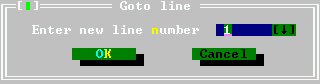
\epsfig{file=pics/ide/gotoline.png}
\else
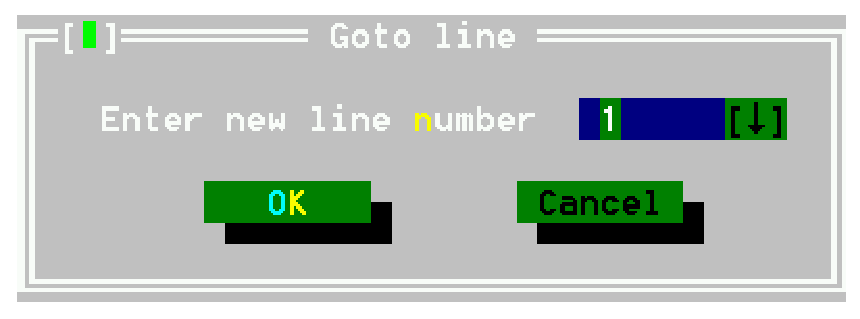
\epsfig{file=pics/ide/gotoline.eps}
\fi
\end{center}
\end{figure}
\end{latexonly}


%
% Syntax highlighting and code completion
%
\subsection{Syntax highlighting}
\label{se:syntaxhighlighting}
The IDE is capable of syntax highlighting, i.e. the color of certain 
Pascal elements can be set. As text is entered in an editor window, 
the IDE will try to recognise the elements, and set the color of the
text accordingly.


The syntax highlighting can be customized in the colors preferences dialog,
using the menu option \menu{Options|\-Environment|\-Colors}. In the colors dialog, the
group "Syntax" must be selected. The item list will then display the 
various syntactical elements that can be colored:
\begin{description}
\item[Whitespace] The empty text between words. Remark that for whitespace,
only the background color will be used.
\item[Comments] All styles of comments in Free Pascal.
\item[Reserved words] All reserved words of Free Pascal. (see also \refref).
\item[Strings] Constant string expressions.
\item[Numbers] Numbers in decimal notation.
\item[Hex numbers] Numbers in hexadecimal notation.
\item[Assembler] Any assembler blocks.
\item[Symbols] Recognised symbols (variables, types)
\item[Directives] Compiler directives.
\item[Tabs] Tab characters in the source can be given a different color than 
other whitespace.
\end{description}
The editor uses some default settings, but experimentation is the best way
to find a fitting color scheme. A good color scheme helps detecting errors
in sources, since errors will result in wrong syntax highlighting. 

% Code completion
\subsection{Code Completion}
\label{se:codecompletion}
Code completion means the editor will try to guess the text as it
is being typed. It does this by checking what text is typed, and as soon
as the typed text can be used to identify a keyword in a list of keywords,
the keyword will be presented in a small colored box under the typed text. 
Pressing the \key{Enter} key will complete the word in the text.

There is no code completion yet for filling in function arguments, choosing
object methods as in e.g. \delphi.

Code completion can be customized in the Code completion dialog, reachable 
through the menu option \menu{Options|\-Preferences|\-Codecompletion}.
The list of keywords that can be completed can be maintained here. 

\begin{htmlonly}
The code completion dialog.
\fpcaddimg{../pics/ide/codecomp.png}
\end{htmlonly}
\begin{latexonly}
The code completion dialog is shown in \seefig{codecomp}.
\begin{figure}[ht]
\begin{center}
\caption{The code completion dialog.}\label{fig:codecomp}
\ifpdf
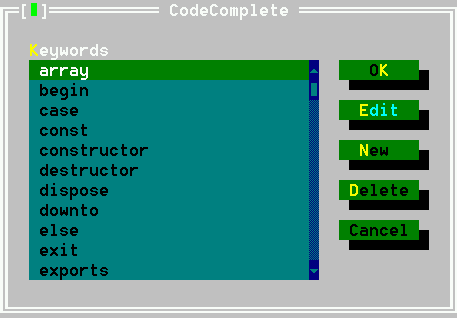
\epsfig{file=pics/ide/codecomp.png}
\else
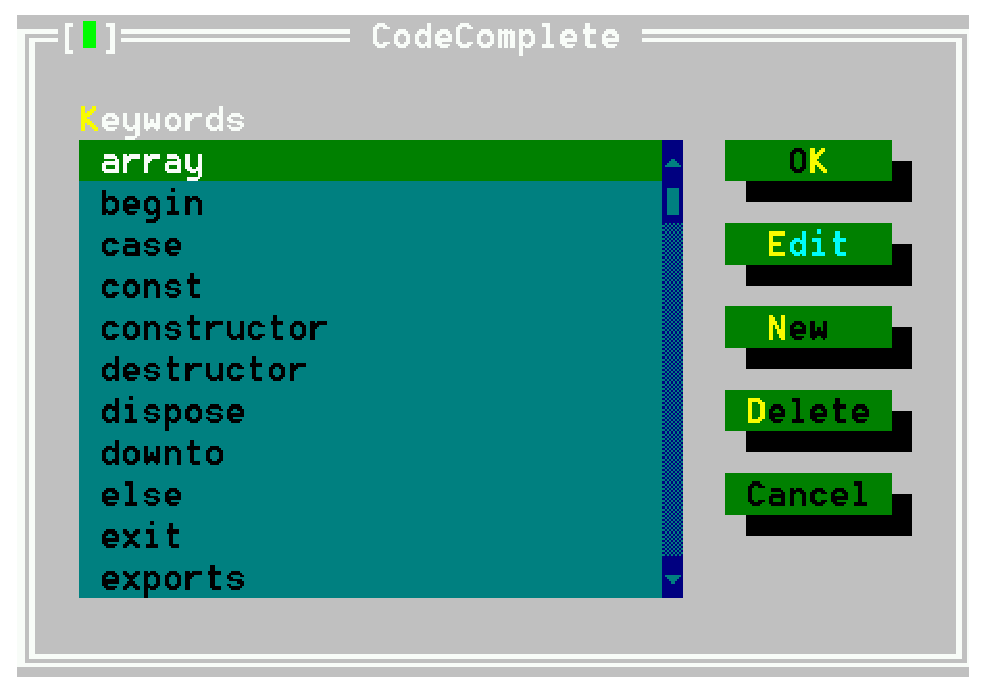
\epsfig{file=pics/ide/codecomp.eps}
\fi
\end{center}
\end{figure}
\end{latexonly}
The dialog shows the currently defined keywords that will be completed in
alphabetical order.
The following buttons are available:
\begin{description}
\item[Ok] Saves all changes and closes the dialog.
\item[Edit] Pops up a dialog that allows to edit the currently 
highlighted keyword.
\item[New] Pops up a dialog that allows to enter a new keyword which will be
added to the list.
\item[Delete] Deletes the currently highlighted keyword from the list
\item[Cancel] Discards all changes and closes the dialog.
\end{description}
All keywords are saved and are available the next time the IDE is started.
Duplicate names are not allowed. If an attempt is made to add a duplicate
name to the list, an error will follow.

% Code templates
\subsection{Code Templates}
Code templates are a way to insert large pieces of code at once. Each 
code templates is identified by a unique name. This name can be used to
insert the associated piece of code in the text.

For example, the name \var{ifthen} could be associated to the following
piece of code:
\begin{verbatim}
If | Then
  begin
  end
\end{verbatim}
A code template can be inserted by typing its name, and pressing \key{Ctrl-J}
when the cursor is positioned right after the template name.

If there is no template name before the cursor, a dialog will pop up to
allow selection of a template.

If a vertical bar (|) is present in the code template, the cursor is positioned
on it, and the vertical bar is deleted. In the above example, the cursor would be
positioned between the \var{if} and \var{then}, ready to type an expression.

Code templates can be added and edited in the code templates dialog, reachable via
the menu option \menu{Options|\-Preferences|\-Codetemplates}. 

\begin{htmlonly}
The code templates dialog.
\fpcaddimg{../pics/ide/codetemp.png}
\end{htmlonly}
\begin{latexonly}
The code templates dialog is shown in \seefig{codetemp}.
\begin{figure}[ht]
\begin{center}
\caption{The code templates dialog.}\label{fig:codetemp}
\ifpdf
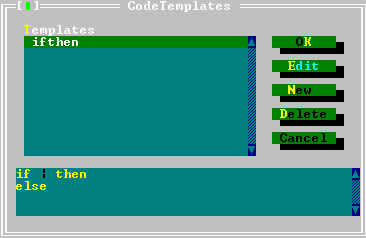
\epsfig{file=pics/ide/codetemp.png}
\else
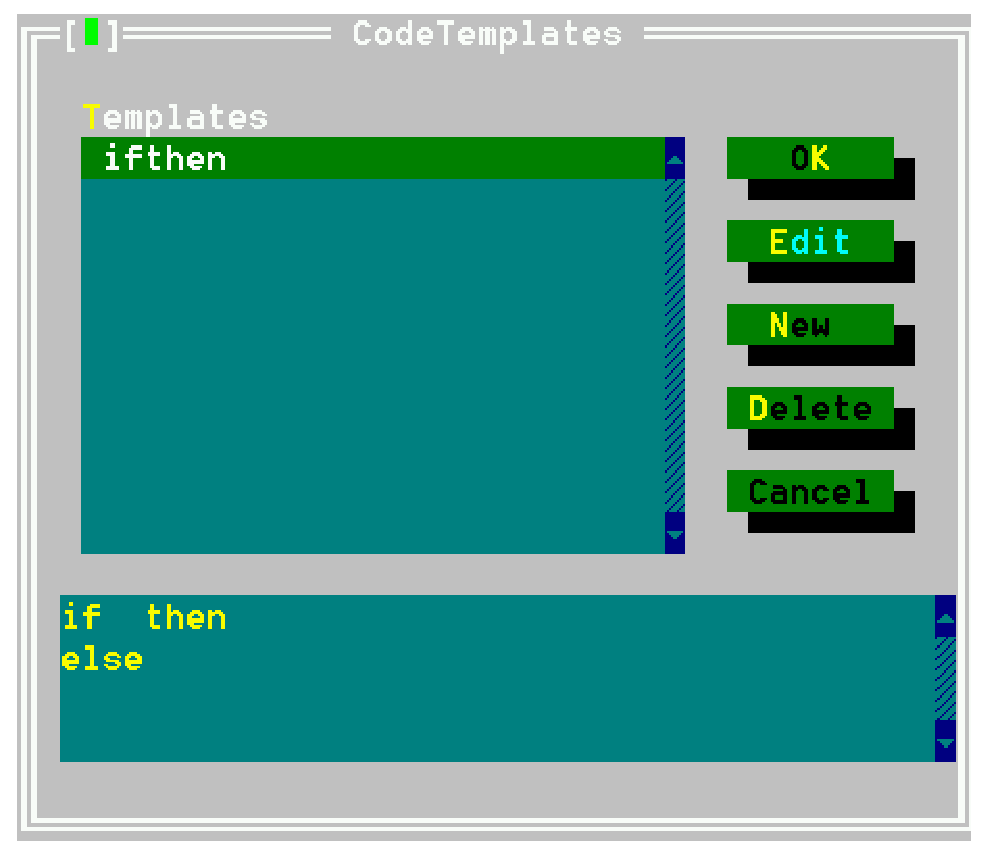
\epsfig{file=pics/ide/codetemp.eps}
\fi
\end{center}
\end{figure}
\end{latexonly}
The top listbox in the code templates dialog shows the names of all 
known templates. The bottom half of the dialog shows the text associated
with the currently highlighted code template.
The following buttons are available:
\begin{description}
\item[Ok] Saves all changes and closes the dialog.
\item[Edit] Pops up a dialog that allows to edit the currently 
highlighted code template. Both the name and text can be edited.
\item[New] Pops up a dialog that allows to enter a new code template
which will be added to the list. A name must be entered for the new
template.
\item[Delete] Deletes the currently highlighted code template from the list
\item[Cancel] Discards all changes and closes the dialog.
\end{description}
All templates are saved and are available the next time the IDE is started.
\begin{remark}
Duplicates are not allowed. If an attempt is made to add a duplicate name
to the list, an error will occur.
\end{remark}

%%%%%%%%%%%%%%%%%%%%%%%%%%%%%%%%%%%%%%%%%%%%%%%%%%%%%%%%%%%%%%%%%%%%%%%
% Searching in the text
\section{Searching and replacing}
\label{se:searching}
The IDE allows to search for text in the active editor window. 
To search for text, one of the following can be done:
\begin{enumerate}
\item Select \menu{Search|Find} in the menu.
\item Press \key{Ctrl-Q F}.
\end{enumerate}
\begin{htmlonly}
After that, the following dialog will pop up:
\fpcaddimg{../pics/ide/search.png}
In this dialog, the following options can be entered:
\end{htmlonly}
\begin{latexonly}
After that, the dialog shown in \seefig{search} will pop up,
and the following options can be entered
\begin{figure}[ht]
\caption{The search dialog.}\label{fig:search}
\ifpdf
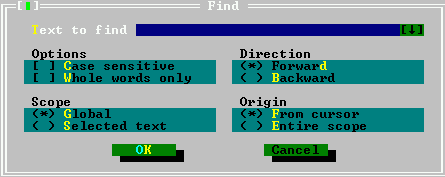
\epsfig{file=pics/ide/search.png,width=\textwidth}
\else
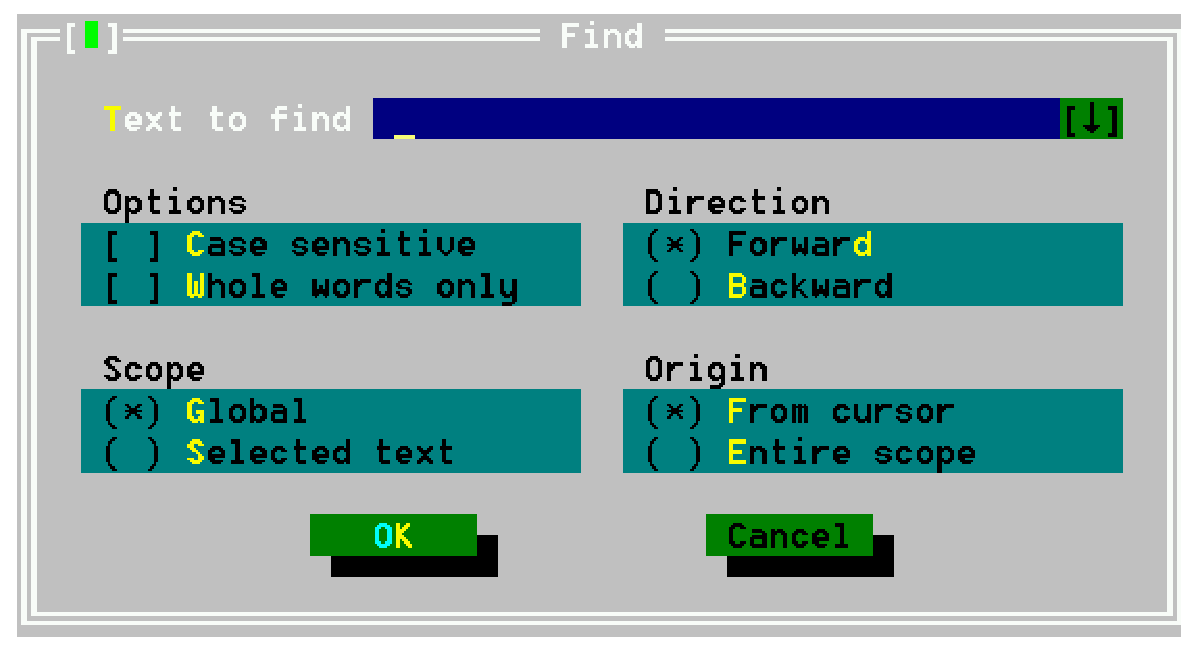
\epsfig{file=pics/ide/search.eps,width=\textwidth}
\fi
\end{figure}
\end{latexonly}

\begin{description}
\item[Text to find] The text to be searched for. If a block was active when
the dialog was started, the first line of this block is proposed.
\item[Case sensitive] When checked, the search is case sensitive.
\item[Whole words only] When checked, the search text must appear in the
text as a complete word.
\item[Direction] The direction in which the search must be conducted,
starting from the specified origin.
\item[Scope] Specifies if the search should be on the whole file, or just the selected
text.
\item[Origin] Specifies if the search should start from the cursor position or the start
of the scope.
\end{description}
After the dialog has closed, the search is performed using the given options.

A search can be repeated (using the same options) in one of 2 ways:
\begin{enumerate}
\item Select \menu{Search|Find again} from the menu.
\item Press \key{Ctrl-L}.
\end{enumerate}

It is also possible to replace occurrences of a text with another text. 
This can be done in a similar manner to searching for a text:
\begin{enumerate}
\item Select \menu{Search|Replace} from the menu.
\item Press \key{Ctrl-Q A}.
\end{enumerate}
A dialog, similar to the search dialog will pop up:
\begin{htmlonly}
A dialog, similar to the search dialog will pop up:
\fpcaddimg{../pics/ide/replace.png}
In this dialog, the following options can be entered:
\end{htmlonly}
\begin{latexonly}
A dialog, similar to the search dialog will pop up, as shown in \seefig{replace}.
\begin{figure}[ht]
\caption{The replace dialog.}\label{fig:replace}
\ifpdf
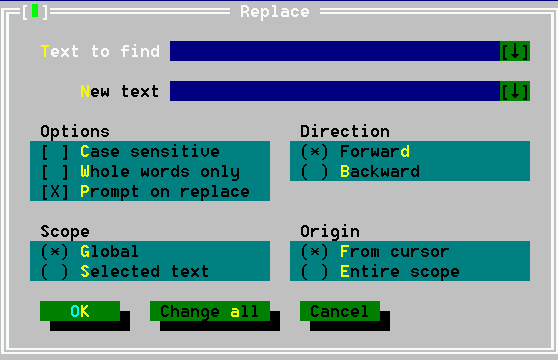
\epsfig{file=pics/ide/replace.png,width=\textwidth}
\else
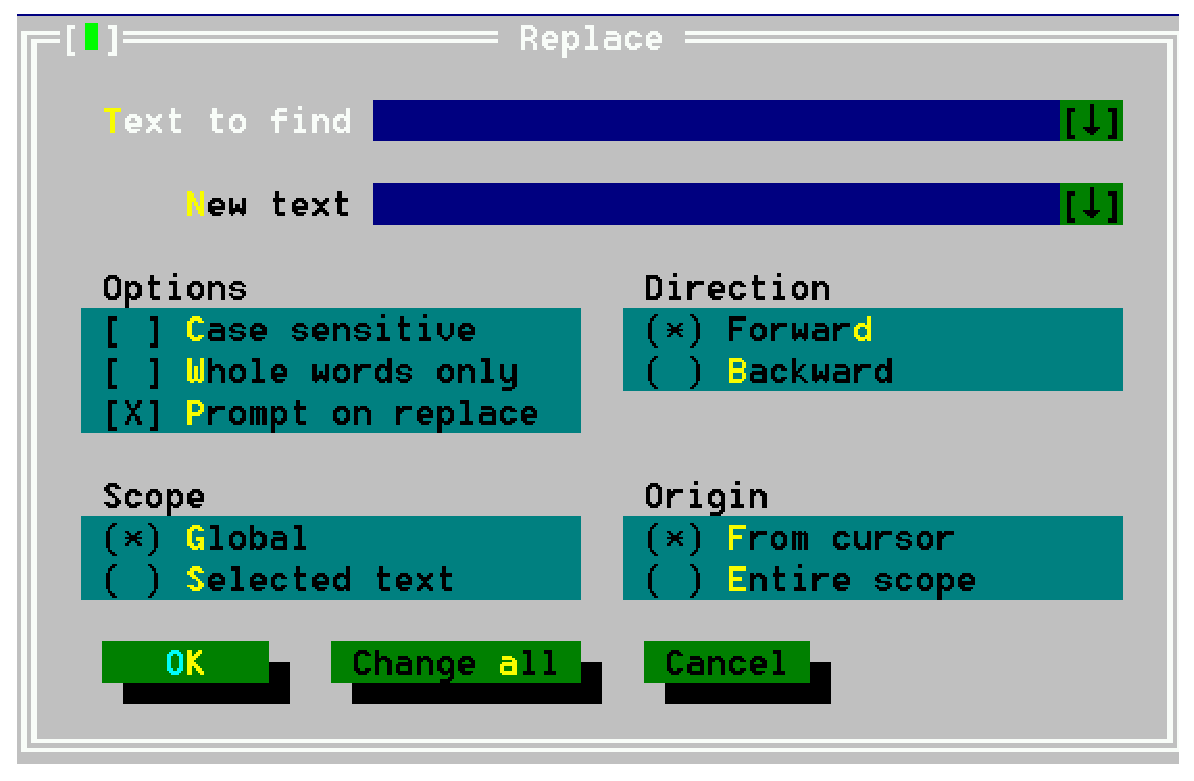
\epsfig{file=pics/ide/replace.eps,width=\textwidth}
\fi
\end{figure}
\end{latexonly}

In this dialog, in addition to the things that can be filled in in the
search dialog, the following things can be entered:
\begin{description}
\item [New text] Text by which found text will be replaced.
\item [Prompt on replace] Before a replacement is made, the IDE will ask for
confirmation.
\end{description}
If the dialog is closed with the 'OK' button, only the next occurrence of
the the search text will be replaced. 
If the dialog is closed with the 'Change All' button, all occurrences of 
the search text will be replaced.

%%%%%%%%%%%%%%%%%%%%%%%%%%%%%%%%%%%%%%%%%%%%%%%%%%%%%%%%%%%%%%%%%%%%%%%
% The symbol browser
\section{The symbol browser}
\label{se:browser}
The symbol browser allows to find all occurrences of a symbol. A symbol 
can be a variable, type, procedure or constant that occurs in the
program or unit sources.

To enable the symbol browser, the program or unit must be compiled with
browser information. This can be done by setting the browser information
options in the compiler options dialog.

The IDE allows to browse several types of symbols:
\begin{description}
\item[procedures] Allows to quickly jump to a procedure definition or
implementation.
\item[Objects] Allows to quickly browse an object.
\item[Modules] Allows to browse a module.
\item[Globals] Allows to browse any global symbol.
\item[Arbitrary symbol] Allows to browse an arbitrary symbol.
\end{description}
In all cases, first a symbol to be browsed must be selected. After that,
a browse window appears. In the browse window, all locations where the 
symbol was encountered are shown. Selecting a location and pressing the
space bar will cause the editor to jump to that location; the line
containing the symbol will be highlighted. 

If the location is in a source file that is not yet displayed, a new 
window will be opened with the source file loaded.

After the desired location was reached, the browser window can be closed 
with the usual commands. 

The behaviour of the browser can be customized with the browser options
dialog, using the \menu{Options|Browser} menu.
\begin{htmlonly}
The browser options dialog looks as follows:
\fpcaddimg{../pics/ide/obrowser.png}
\end{htmlonly}
\begin{latexonly}
The browser options dialog looks like \seefig{obrowser}.
\begin{figure}[ht]
\caption{The browser options dialog.}\label{fig:obrowser}
\ifpdf
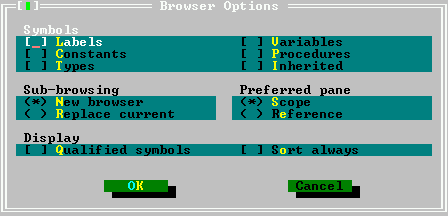
\epsfig{file=pics/ide/obrowser.png,width=\textwidth}
\else
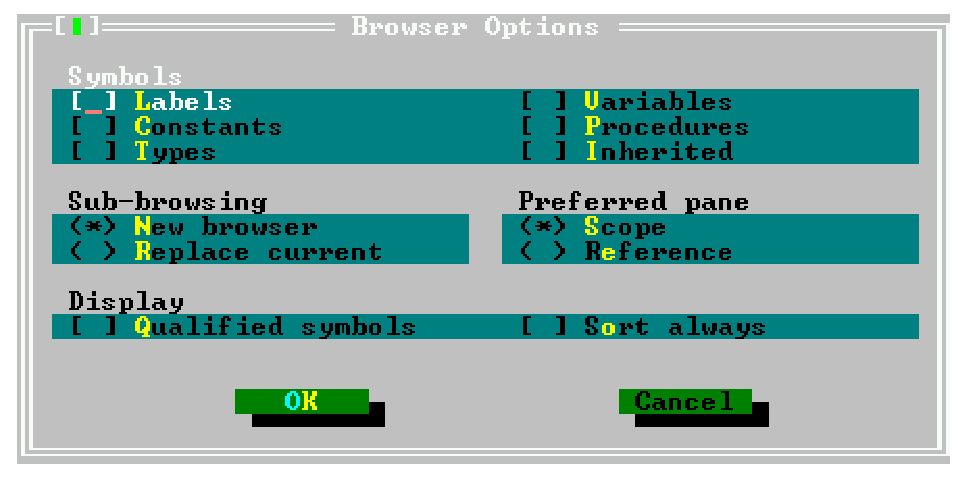
\epsfig{file=pics/ide/obrowser.eps,width=\textwidth}
\fi
\end{figure}
\end{latexonly}
The following options can be set in the browser options dialog:
\begin{description}
\item[Symbols] Here the types of symbols displayed in the browser can be
selected:
\begin{description}
\item[Labels] labels are shown.
\item[Constants] Constants are shown.
\item[Types] Types are shown.
\item[Variables] Variables are shown.
\item[Procedures] Procedures are shown.
\item[Inherited]
\end{description}
\item[Sub-browsing] Specifies what the browser should do when displaying the
members of a complex symbol such as a record or class:
\begin{description}
\item[New browser] The members are shown in a new browser window.
\item[Replace current] The contents of the current window are replaced with
the members of the selected complex symbol.
\end{description}
\item[Preferred pane] Specifies what pane is shown in the browser when it is
initially opened:
\begin{description}
\item[scope]
\item[Reference]
\end{description}
\item[Display] Determines how the browser should display the symbols:
\begin{description}
\item[Qualified symbols]
\item[Sort always] sorts the symbols in the browser window. 
\end{description}
\end{description}

%%%%%%%%%%%%%%%%%%%%%%%%%%%%%%%%%%%%%%%%%%%%%%%%%%%%%%%%%%%%%%%%%%%%%%%
% Running programs
\section{Running programs}
\label{se:running}
A compiled program can be run straight from the IDE. This can be done
in one of several ways:
\begin{enumerate}
\item select the \menu{Run|Run} menu, or
\item press \key{Ctrl-F9}.
\end{enumerate}
If command-line parameters should be passed to the program, then these
can be set through the \menu{Run|Parameters} menu. 
\begin{htmlonly}
The Parameters dialog.
\fpcaddimg{../pics/ide/params.png}
\end{htmlonly}
\begin{latexonly}
The program parameters dialog looks like \seefig{params}.
\begin{figure}[ht]
\caption{The program parameters dialog.}\label{fig:params}
\ifpdf
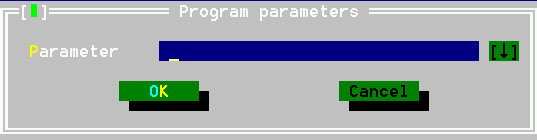
\epsfig{file=pics/ide/params.png,width=\textwidth}
\else
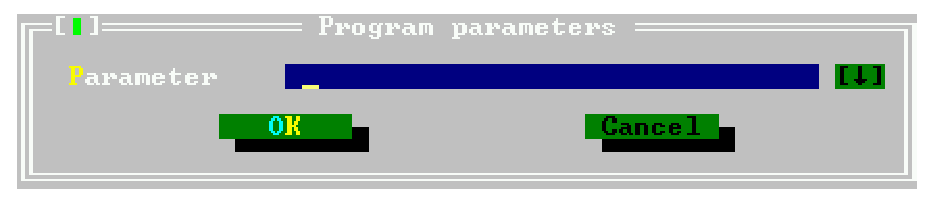
\epsfig{file=pics/ide/params.eps,width=\textwidth}
\fi
\end{figure}
\end{latexonly}

Once the program started, it will continue to run, until 
\begin{enumerate}
\item the program quits normally,
\item an error happens,
\item a breakpoint is encountered or
\item the program is reset by the user.
\end{enumerate}
The last alternative is only possible if the program is compiled
with debug information.

Alternatively, it is possible to position the cursor somewhere in a
source file, and run the program till the execution reaches the
source-line where the cursor is located. This can be done by
\begin{enumerate}
\item selecting \menu{Run|Goto Cursor} in the menu,
\item pressing \key{F4}.
\end{enumerate}
Again, this is only possible if the program was compiled with debug
information.

The program can also executed line by line. Pressing \key{F8} will 
execute the next line of the program. If the program wasn't started
yet, it is started. Repeatedly pressing \key{F8} will execute line 
by line of the program, and the IDE will show the line to be executed 
in an editor window. If somewhere in the code a call occurs to a subroutine,
then pressing \key{F8} will cause the whole routine to be executed before
control returns to the IDE. If the code of the subroutine should be stepped
through as well, then \key{F7} should be used instead. Using \key{F7} will
cause the IDE to execute line by line of any subroutine that is encountered.

If a subroutine is being stepped through, then the \menu{Run|Until return} menu
will execute the program till the current subroutine ends. 

If the program should be stopped before it quits by itself, then this can be
done by
\begin{enumerate}
\item selecting \menu{Run|Program reset} from the menu, or
\item pressing \key{Ctrl-F2}.
\end{enumerate}
The running program will then be aborted.

%%%%%%%%%%%%%%%%%%%%%%%%%%%%%%%%%%%%%%%%%%%%%%%%%%%%%%%%%%%%%%%%%%%%%%%
% Debugging programs
\section{Debugging programs}
\label{se:debugging}
To debug a program, it must be compiled with debug information. Compiling a
program with debug information allows to:
\begin{enumerate}
\item Execute the program line by line.
\item Run the program till a certain point (a breakpoint)
\item Inspect the contents of variables or memory locations while the
program is running.
\end{enumerate}
%
% Using breakpoints
%
\subsection{Using breakpoints}
Breakpoints will cause a running program to stop when the execution
reaches the line where the breakpoint was set. At that moment, control
is returned to the IDE, and it is possible to continue execution.

To set a breakpoint on the current source line, use the 
\menu{Debug|Breakpoint} menu entry, or press \key{Ctrl-F8}.

A list of current breakpoints can be obtained through the
\menu{Debug|Breakpoint list} menu. 
\begin{htmlonly}
The breakpoint list window looks as follows:
\fpcaddimg{../pics/ide/brklist.png}
\end{htmlonly}
\begin{latexonly}
The breakpoint list window is shown in \seefig{brklist}
\begin{figure}[ht]
\caption{The breakpoint list window.}\label{fig:brklist}
\ifpdf
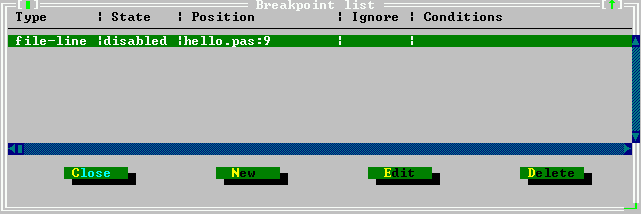
\epsfig{file=pics/ide/brklist.png,width=\textwidth}
\else
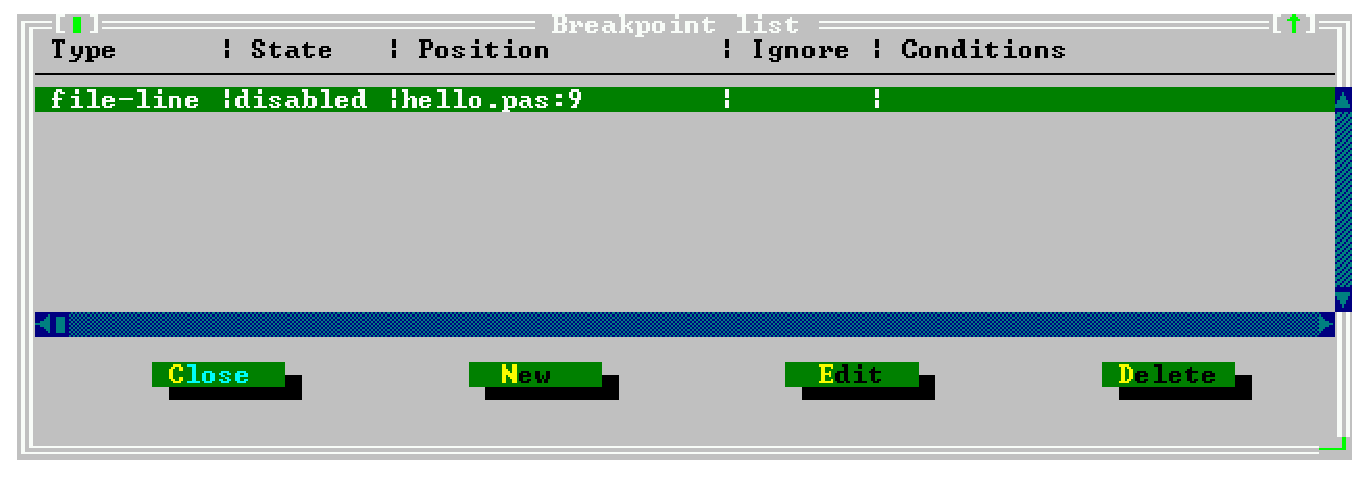
\epsfig{file=pics/ide/brklist.eps,width=\textwidth}
\fi
\end{figure}
\end{latexonly}
In the breakpoint list window, the following things can be done:
\begin{description}
\item[New] Shows the breakpoint property dialog where the properties
for a new breakpoint can be entered. 
\item[Edit] Shows the breakpoint property dialog where the properties of
the highlighted breakpoint can be changed. 
\item[Delete] Deletes the highlighted breakpoint.
\end{description}
The dialog can be closed with the 'Close' button.

\begin{htmlonly}
The breakpoint properties dialog looks as follows:
\fpcaddimg{../pics/ide/brkprop.png}
\end{htmlonly}
\begin{latexonly}
The breakpoint properties dialog is shown in \seefig{brkprop}
\begin{figure}[ht]
\caption{The breakpoint properties dialog.}\label{fig:brkprop}
\ifpdf
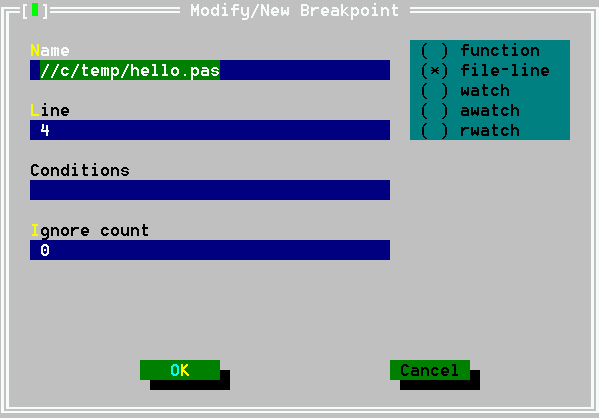
\epsfig{file=pics/ide/brkprop.png,width=\textwidth}
\else
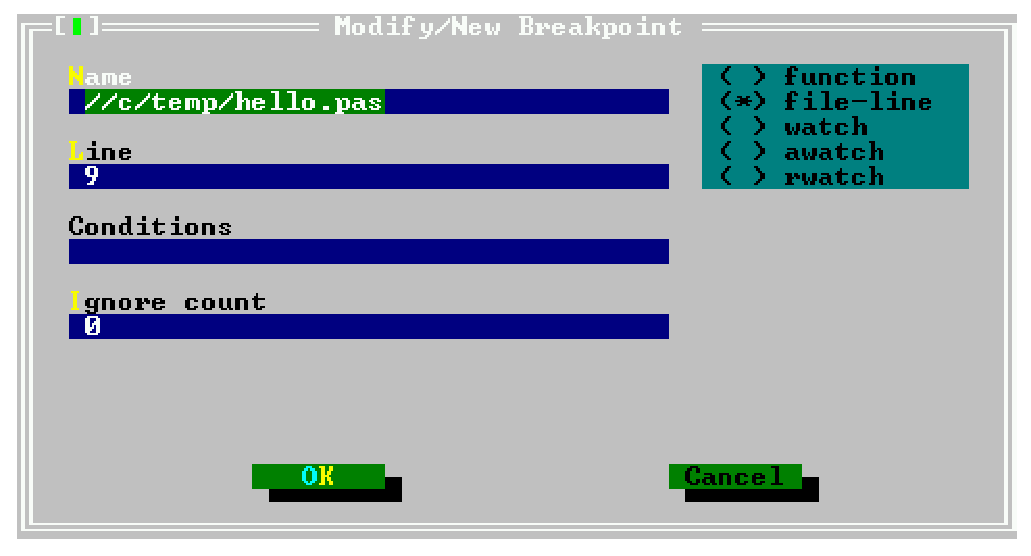
\epsfig{file=pics/ide/brkprop.eps,width=\textwidth}
\fi
\end{figure}
\end{latexonly}
The following properties can be set:
\begin{description}
\item[type]
\begin{description}
\item[function] function breakpoint. The program will stop when the function
with the given name is reached.
\item[file-line] Source line breakpoint. The program will stop when the
source file with given name and line is reached;
\item[watch] Expression breakpoint. An expression may be entered, and the
program will stop as soon as the expression changes.
\item[awatch] (access watch) Expression breakpoint. An expression that references a 
memory location may be entered, and the program will stop as soon as 
the memory indicated by the expression is accessed.
\item[rwatch] (read watch) Expression breakpoint. An expression that references a
memory location may be entered, and the program will stop as soon as 
the memory indicated by the expression is read.
\end{description}
\item[name] Name of the function or file where to stop.
\item[line] Line number in the file where to stop. Only for breakpoints of
type file-line.
\item[Conditions] Here an expression can be entered which must evaluate 
\var{True} for the program to stop at the breakpoint. The expressions that
can be entered must be valid GDB expressions.
\item[Ignore count] The number of times the breakpoint will be ignored
before the program stops; 
\end{description}
\begin{remark}
\begin{enumerate}
\item Because the IDE uses GDB to do its debugging, it is necessary to enter all
expressions in {\em uppercase} on \freebsd. 
\item Expressions that reference memory locations should be no longer than 16 
bytes on \linux or go32v2 on an Intel processor, since the Intel processor's 
debug registers are used to monitor these locations.
\item Memory location watches will not function on Win32 unless a special 
patch is applied. 
\end{enumerate}
\end{remark}

%
% Using watches
%
\subsection{Using watches}
When debugging information is compiled in the program, watches can be used.
Watches are expressions which can be evaluated by the IDE and shown in a
separate window. When program execution stops (e.g. at a breakpoint) all
watches will be evaluated and their current values will be shown.

Setting a new watch can be done with the \menu{Debug|Add watch} menu 
command or by pressing \key{Ctrl-F7}. When this is done, the watch
property dialog appears, and a new expression can be entered.
\begin{htmlonly}
The watch property dialog looks as follows:
\fpcaddimg{../pics/ide/watch.png}
\end{htmlonly}
\begin{latexonly}
The watch property dialog is shown in \seefig{watch}
\begin{figure}[ht]
\begin{center}
\caption{The watch property dialog.}\label{fig:watch}
\ifpdf
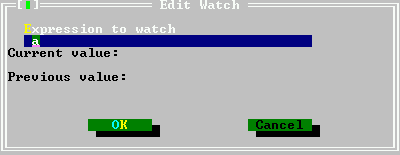
\epsfig{file=pics/ide/watch.png}
\else
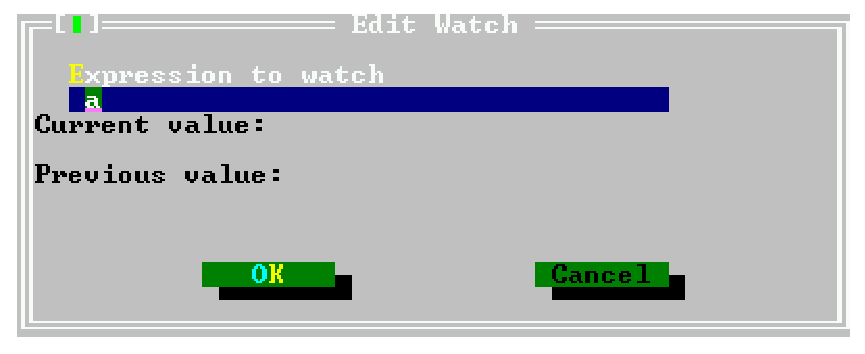
\epsfig{file=pics/ide/watch.eps}
\fi
\end{center}
\end{figure}
\end{latexonly}
In the dialog, the expression can be entered, any possible previous value
and current value are shown.
\begin{remark}
Because the IDE uses GDB to do it's debugging, it is necessary to enter all
expressions in {\em uppercase} in \freebsd. 
\end{remark}
A list of watches and their present value is available in the watches
window, which can be opened with the \menu{Debug|Watches} menu.
\begin{htmlonly}
The watch list window looks as follows:
\fpcaddimg{../pics/ide/watchlst.png}
\end{htmlonly}
\begin{latexonly}
The watch list window is shown in \seefig{brklist}
\begin{figure}[ht]
\begin{center}
\caption{The watch list window.}\label{fig:watchlst}
\ifpdf
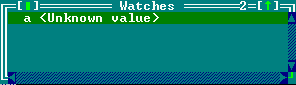
\epsfig{file=pics/ide/watchlst.png}
\else
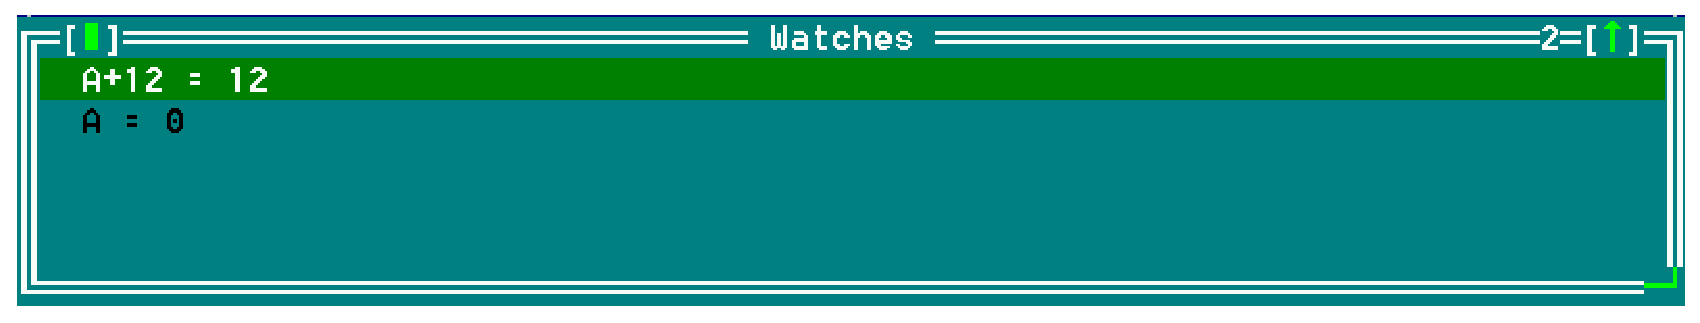
\epsfig{file=pics/ide/watchlst.eps}
\fi
\end{center}
\end{figure}
\end{latexonly}

Pressing \key{Enter} or the space bar will show the watch property dialog
for the currently highlighted watch in the watches window.

The list of watches is updated whenever the IDE resumes control when
debugging a program.
%
% The call stack
%
\subsection{The call stack}
\label{se:callstack}
The call stack helps in showing the program flow. It shows the list of
procedures that are being called at this moment, in reverse order.
The call stack window can be shown using the \menu{Debug|Call Stack}
It will show the address or procedure name of all currently active 
procedures with their filename and addresses. If parameters were passed
they will be shown as well.
\begin{htmlonly}

The call stack window looks as follows:
\fpcaddimg{../pics/ide/callstck.png}
\end{htmlonly}
\begin{latexonly}
The call stack is shown in \seefig{callstack}.
\begin{figure}[ht]
\begin{center}
\caption{The call stack window.}\label{fig:callstack}
\ifpdf
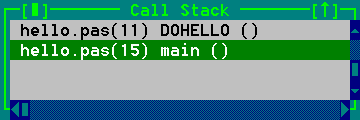
\epsfig{file=pics/ide/callstck.png}
\else
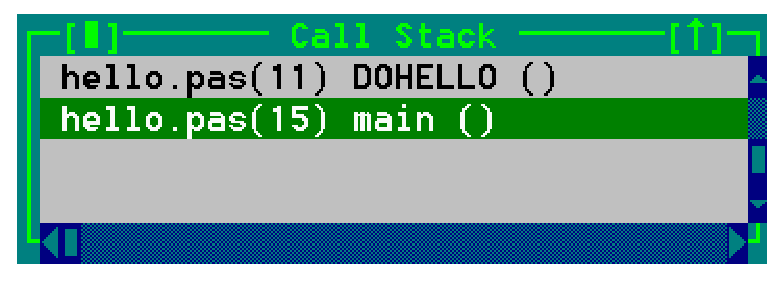
\epsfig{file=pics/ide/callstck.eps}
\fi
\end{center}
\end{figure}
\end{latexonly}

By pressing the space bar in the call stack window, the line corresponding
to the call will be highlighted in the edit window.

% The GDB Window
\subsection{The GDB window}
\label{se:gdbwindow}
The GDB window provides direct interaction with the GDB debugger.
In it, GDB commands can be typed as they would be typed in GDB.
The response of GDB will be shown in the window.

Some more information on using GDB can be found in \sees{usinggdb}, but
the final reference is of course the GDB manual itself
\footnote{Available from the Free Software Foundation website.}.

\begin{htmlonly}
The GDB window looks as follows:
\fpcaddimg{../pics/ide/gdbwin.png}
\end{htmlonly}
\begin{latexonly}
The GDB window is shown in \seefig{gdbwin}.
\begin{figure}[ht]
\begin{center}
\caption{The GDB window.}\label{fig:gdbwin}
\ifpdf
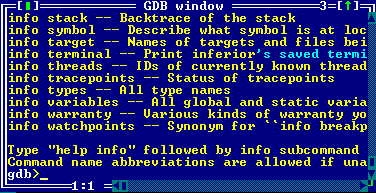
\epsfig{file=pics/ide/gdbwin.png}
\else
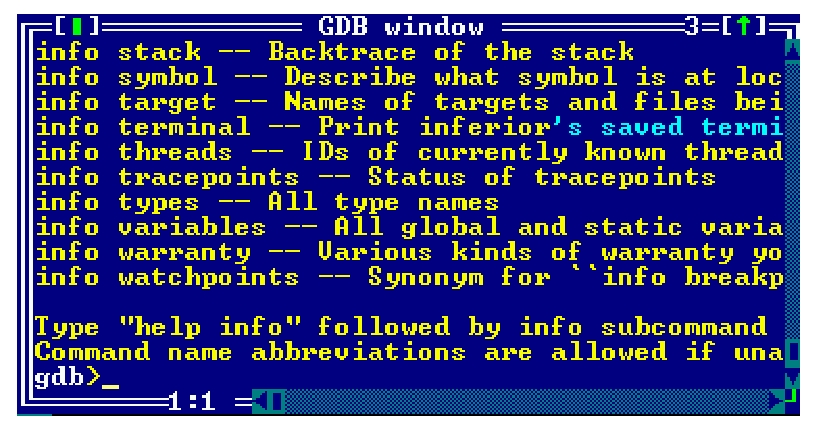
\epsfig{file=pics/ide/gdbwin.eps},
\fi
\end{center}
\end{figure}
\end{latexonly}

%%%%%%%%%%%%%%%%%%%%%%%%%%%%%%%%%%%%%%%%%%%%%%%%%%%%%%%%%%%%%%%%%%%%%%%
% The tools menu
\section{Using Tools}
\label{se:toolsmenu}
The tools menu provides easy access to external tools. It also has
three pre-defined tools for programmers: an ASCII table,  a grep tool
and a calculator. The output of the external tools can be accessed through
this menu as well.

%
% The messages window.
%
\subsection{The messages window}
\label{se:toolsmessages}
The output of the external utilities is redirected by the IDE and it
will be displayed in the messages window. The messages window is
displayed automatically, if an external tool was run. The
messages window can be also displayed manually by the selecting the
menu item \menu{Tools|Messages} or by pressing the key \key{F11}.

\begin{htmlonly}
The messages window looks as follows:
\fpcaddimg{../pics/ide/messages.png}
\end{htmlonly}
\begin{latexonly}
The messages window is shown in \seefig{messages}.
\begin{figure}[ht]
\caption{The messages window.}\label{fig:messages}
\ifpdf
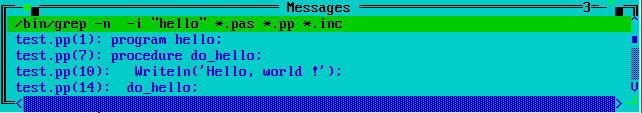
\epsfig{file=pics/ide/messages.png,width=\textwidth}
\else
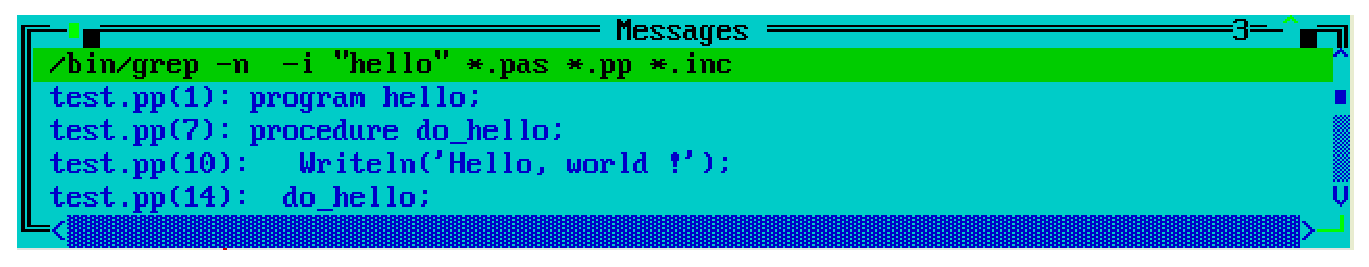
\epsfig{file=pics/ide/messages.eps,width=\textwidth}
\fi
\end{figure}
\end{latexonly}
If the output of the tool contains filenames and line numbers,
the messages window can be used to navigate the source as in a browse
window:
\begin{enumerate}
\item Pressing \key{Enter} or double clicking the output line will jump
to the specified source line and close the messages window.
\item Pressing the space bar will jump to the specified source line, but
will leave the messages window open, with the focus on it. This allows to
quickly select another message line with the arrow keys and jump to 
another location in the sources.
\end{enumerate}
The algorithm which extracts the file names and line numbers from
the tool output is quite sophisticated, but in some cases it may
fail\footnote{Suggestions for improvement, or better yet, patches
that improve the algorithm, are always welcome.}.
%
% Grep
%
\subsection{Grep}
\label{se:grep}
One external tool in the Tools menu is already predefined: a
menu item to call the \file{grep} utility (\menu{Tools|Grep} or
\key{Shift-F2}). \file{Grep} searches for a given string in files and
returns the lines which contain the string. The search string can
be even a regular expression. For this menu item to work, the
\file{grep} program must be installed, since it does not come with \fpc.

The messages window displayed in \seefig{messages} in the previous 
section shows the output of a typical \file{grep} session. The messages
window can be used in combination with \file{grep} to find special
occurrences in the text.

\file{Grep} supports regular expressions. A regular expression is a 
string with special characters which describe a whole class of 
expressions. The command line in \dos or \linux have limited 
support for regular expressions: entering \var{ls *.pas} 
(or \var{dir *.pas}) to get a list of all Pascal files in a
directory. \file{*.pas} is something similar to a regular expression. 
It uses a wildcard to describe a whole class of strings: those which 
end on "\file{.pas}". 
Regular expressions offer much more: for example \var{[A-Z][0-9]+} 
describes all strings which begin with a upper case letter followed by
one or more digits.

It is outside the scope of this manual to describe regular expressions
in great detail. Users of a \linux system can get more information on grep
using \var{man grep} on the command-line.
%
% The ASCII table.
%
\subsection{The ASCII table}
\label{se:asciitable}
The tools menu provides also an ASCII table (\menu{Tools|Ascii table}),
The ASCII table can be used to look up ASCII codes as well as
inserting characters into the window which was active when invoking the
table. To get the ASCII code of a char move the cursor on this char 
or click with the mouse on it. To insert a
char into an editor window either:
\begin{enumerate}
\item using the mouse, double click it,
\item using the keyboard,  press \key{Enter} while the cursor is on it.
\end{enumerate}
This is especially useful for pasting graphical characters in a constant
string.

The ASCII table remains active till another window is explicitly activated,
thus multiple characters can be inserted at once.
\begin{htmlonly}
The ASCII table looks as follows:
\fpcaddimg{../pics/ide/ascii.png}
\end{htmlonly}
\begin{latexonly}
The ASCII table is shown in \seefig{asciitable}.
\begin{figure}[ht]
\begin{center}
\caption{The ASCII table.}\label{fig:asciitable}
\ifpdf
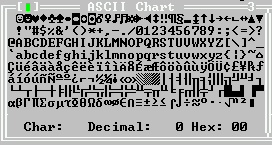
\epsfig{file=pics/ide/ascii.png}
\else
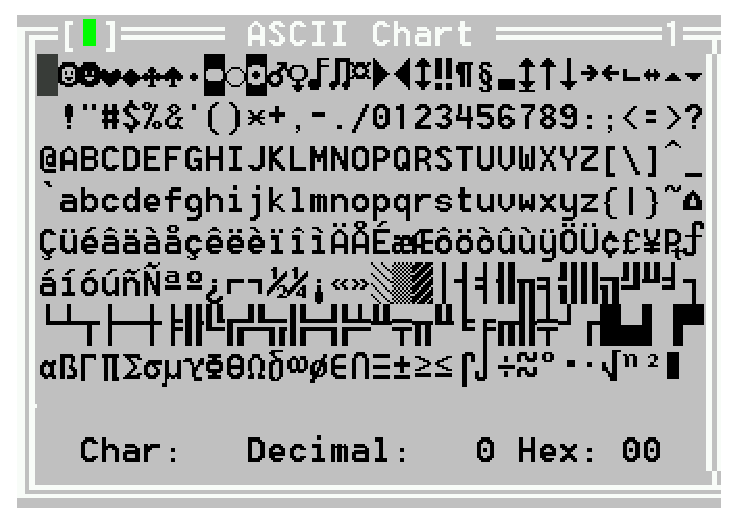
\epsfig{file=pics/ide/ascii.eps}
\fi
\end{center}
\end{figure}
\end{latexonly}

%
% The calculator
%
\subsection{The calculator}
\label{se:calculator}
The calculator allows to do some quick calculations. It is a simple
calculator, since it does not take care of operator precedence, and
bracketing of operations is not (yet) supported.

The result of the calculations can be pasted into the text using the
\key{Ctrl-Enter} keystroke.

\begin{htmlonly}
The calculator dialog looks as follows:
\fpcaddimg{../pics/ide/calc.png}
\end{htmlonly}
\begin{latexonly}
The calculator dialog is shown in \seefig{calculator}.
\begin{figure}[ht]
\begin{center}
\caption{The calculator dialog.}\label{fig:calculator}
\ifpdf
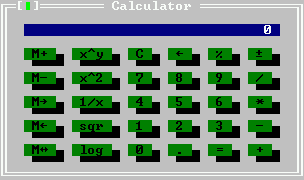
\epsfig{file=pics/ide/calc.png}
\else
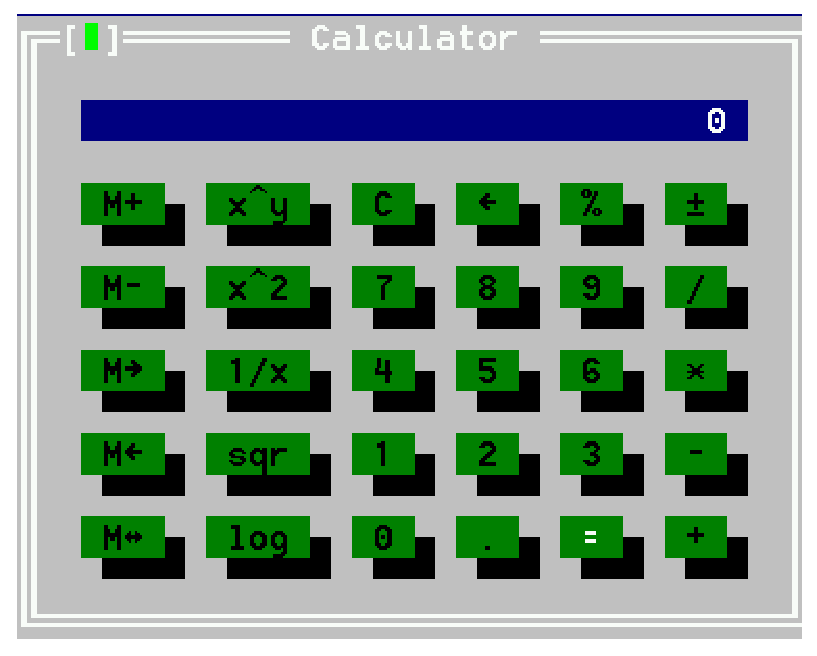
\epsfig{file=pics/ide/calc.eps}
\fi
\end{center}
\end{figure}
\end{latexonly}
The calculator supports all basic mathematical operations such as
addition, subtraction, division and multiplication. They are summarised in
\seet{calculatorbasic}.
\begin{FPCltable}{p{8cm}lll}{Advanced calculator commands}{calculatorbasic}
Operation & Button & Key \\ \hline
Add two numbers & \var{+} & \key{+} \\
Subtract two numbers & \var{\-} & \key{\-} \\
Multiply two numbers & \var{*} & \key{*} \\
Divide two numbers & \var{/} & \key{/} \\
Delete the last typed digit & \var{<-} & \key{Backspace} \\
Delete the display & \var{C} & \key{C} \\
Change the sign & \var{+\-} & \\
Do per cent calculation & \var{\%} & \key{\%} \\ \hline
Get result of operation & \var{=} & \key{Enter} \\ \hline
\end{FPCltable}

But also more sophisticated mathematical operations such as exponentiation
and logarithms are supported. The available mathematical calculations are
shown in \seet{calculatoradvanced}.
\begin{FPCltable}{p{8cm}lll}{Advanced calculator commands}{calculatoradvanced}
Operation & Button & Key \\ \hline
Calculate power & \var{x\^y} & \\
Calculate the inverse value & \var{1/x} & \\
Calculate the square root & \var{sqr} & \\
Calculate the natural logarithm &  \var{log} & \\
Square the display contents & \var{x\^2} & \\ \hline.
\end{FPCltable}

Like many calculators, the calculator in the IDE also supports storing
a single value in memory, and several operations can be done on this memory
value. The available operations are listed in \seet{calculatormemory}
\begin{FPCltable}{p{8cm}lll}{Advanced calculator commands}{calculatormemory}
Operation & Button & Key \\ \hline
Add the displayed number to the memory & \var{M+} & \\
Subtract the displayed number from the memory & \var{M-} & \\
Move the memory contents to the display & \var{M->} & \\
Move the display contents to the memory & \var{M<-} & \\
Exchange display and memory contents & \var{M<->} & \\ \hline
\end{FPCltable}
%
% Adding new tools
%
\subsection{Adding new tools}
\label{se:addingtools}
The tools menu can be extended with any external program which is command-line
oriented. The output of such a program will be caught and displayed in the 
messages window.

Adding a tool to the tools menu can be done using the \menu{Options|Tools} menu.
This will display the tools dialog.
\begin{htmlonly}
The tools dialog looks as follows:
\fpcaddimg{../pics/ide/otools.png}
\end{htmlonly}
\begin{latexonly}
The tools dialog is shown in \seefig{otools}.
\begin{figure}[ht]
\begin{center}
\caption{The tools configuration dialog.}\label{fig:otools}
\ifpdf
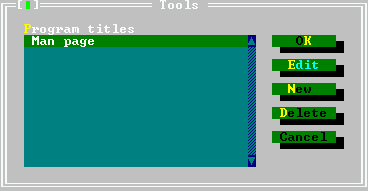
\epsfig{file=pics/ide/otools.png}
\else
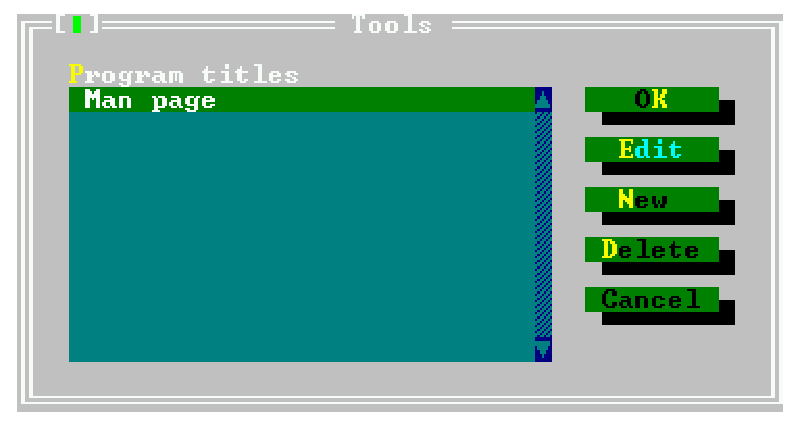
\epsfig{file=pics/ide/otools.eps}
\fi
\end{center}
\end{figure}
\end{latexonly}
In the tools dialog, the following actions are available:
\begin{description}
\item[New] Shows the tool properties dialog where the
properties of a new tool can be entered.
\item[Edit] Shows the tool properties dialog where the
properties of the highlighted tool can be edited.
\item[Delete] Removes the currently highlighted tool.
\item[Cancel] Discards all changes and closes the dialog.
\item[OK] Saves all changes and closes the dialog.
\end{description}
The definitions of the tools are written in the desktop
configuration file, so unless auto-saving of the desktop file
is enabled, the desktop file should be saved explicitly after
the dialog is closed.

\subsection{Meta parameters}
When specifying the command line for the called tool, meta parameters can
be used. Meta parameters are variables and and they are replaced
by their contents before passing the command line to the tool.

\begin{description}
\item[\$CAP]
Captures the output of the tool.
\item[\$CAP\_MSG]
Captures the output of the tool and puts it in the messages window.
\item[\$CAP\_EDIT]
Captures the output of the tool and puts it in a separate editor window.
\item[\$COL]
Replaced by the column of the cursor in the active editor window. If there is no
 active window or the active window is a dialog, then it is replaced by 0.
\item[\$CONFIG]
Replaced by the complete filename of the current configuration file.
\item[\$DIR()]
Replaced by the full directory of the filename argument, including trailing
directory separator. e.g.
\begin{verbatim}
  $DIR('d:\data\myfile.pas')
\end{verbatim}
would return \verb|d:\data\|.
\item[\$DRIVE()]
Replaced by the drive letter of the filename argument. e.g.
\begin{verbatim}
  $DRIVE('d:\data\myfile.pas')
\end{verbatim}
would return \file{d:}.
\item[\$EDNAME]
Replaced by the complete file name of the file in the active edit window.
If there is no active edit window, this is an empty string.
\item[\$EXENAME]
Replaced by the executable name that would be created if the make command
was used. (i.e. from the 'Primary File' setting or the active edit window).
\item[\$EXT()]
Replaced by the extension of the filename argument.
The extension includes the dot.
e.g.
\begin{verbatim}
  $EXT('d:\data\myfile.pas')
\end{verbatim}
would return \file{.pas}.
\item[\$LINE]
Replaced by the line number of the cursor in the active edit window.
If no edit window is present or active, this is 0.
\item[\$NAME()]
Replaced by the name part (excluding extension and dot) of the filename
argument.
e.g.
\begin{verbatim}
  $NAME('d:\data\myfile.pas')
\end{verbatim}
would return \file{myfile}.
\item[\$NAMEEXT()]
Replaced by the name and extension part of the filename argument.
e.g.
\begin{verbatim}
  $NAMEEXT('d:\data\myfile.pas')
\end{verbatim}
would return \file{myfile.pas}.
\item[\$NOSWAP]
Does nothing in the IDE, it is provided for compatibility with \tp only.
\item[\$PROMPT()]
Prompt displays a dialog bow that allows editing of all arguments that
come after it. Arguments that appear before the \var{\$PROMPT} keyword
are not presented for editing.

If a (optional) filename argument is present, \var{\$PROMPT()} will load
a dialog description from the filename argument, e.g.
\begin{verbatim}
$PROMPT(cvsco.tdf)
\end{verbatim}
would parse the file \file{cvsco.tdf}, construct a dialog with it and
display it. After the dialog closed, the information entered by the user
is used to construct the tool command line.

See \sees{commanddialogs} for more information on how to create a dialog
description.
\item[\$SAVE]
Before executing the command, the active editor window is saved, even if it is not modified.
\item[\$SAVE\_ALL]
Before executing the command, all unsaved editor files are saved without prompting.
\item[\$SAVE\_CUR]
Before executing the command the contents of the active editor window are
saved without prompting if they are modified.
\item[\$SAVE\_PROMPT]
Before executing the command, a dialog is displayed asking whether any
unsaved files should be saved before executing the command.
\item[\$WRITEMSG()]
Writes the parsed tool output information to a file with name as in the argument.
\end{description}	

\subsection{Building a command line dialog box}
\label{se:commanddialogs}
When defining a tool, it is possible to show a dialog to the user, asking for
additional arguments, using the \var{\$PROMPT(filename)} command-macro.
\fpc comes with some dialogs, such as a 'grep' dialog, a 'cvs checkout' dialog
and a 'cvs check in' dialog. The files for these dialogs are in the binary
directory and have an extension \file{.tdf}.

In this section, the file format for the dialog description file is explained.
The format of this file resembles a windows \file{.INI} file, where each section
in the file describes an element (or control) in the dialog.
An \var{OK} and an \var{Cancel} button will be added to the bottom of the dialog,
so these should not be specified in the dialog definition.

A special section is the \var{Main} section. It describes how the result of
the dialog will be passed on the command-line, and the total size of the dialog.

\begin{remark}
Keywords that contain a string value, should have the string value enclosed
in double quotes as in
\begin{verbatim}
Title="Dialog title"
\end{verbatim}
\end{remark}

The \var{Main} section should contain the following keywords:
\begin{description}
\item[Title] The title of the dialog. This will appear in the frame title of the dialog.
The string should be enclosed in quotes.
\item[Size] The size of the dialog, this is formatted as \var{(Cols,Rows)}, so
\begin{verbatim}
Size=(59,9)
\end{verbatim}
means the dialog is 59 characters wide, and 9 lines high. This size does not include
the border of the dialog.
\item[CommandLine] specifies how the command-line will be passed to the
program, based on the entries made in the dialog. The text typed here will be passed
on after replacing some control placeholders with their values.

A control placeholder is the name of some control in the dialog, enclosed in
percent (\var{\%}) characters. The name of the control will be replaced with
the text, associated with the control. Consider the following example:
\begin{verbatim}
CommandLine="-n %l% %v% %i% %w% %searchstr% %filemask%"
\end{verbatim}
Here the values associated with the controls named \var{l, i, v, w} and
\var{searchstr} and \var{filemask} will be inserted in the command-line
string.
\item[Default]
The name of the control that is the default control, i.e. the control
that has the focus when the dialog is opened.
\end{description}
The following is an example of a valid main section:
\begin{verbatim}
[Main]
Title="GNU Grep"
Size=(56,9)
CommandLine="-n %l% %v% %i% %w% %searchstr% %filemask%"
Default="searchstr"
\end{verbatim}

After the \var{Main} section, a section must be specified for each control that
should appear on the dialog. Each section has the name of the control it
describes, as in the following example:
\begin{verbatim}
[CaseSensitive]
Type=CheckBox
Name="~C~ase sensitive"
Origin=(2,6)
Size=(25,1)
Default=On
On="-i"
\end{verbatim}
Each control section  must have at least the following keywords associated
with it:
\begin{description}
\item[Type] The type of control. Possible values are:
\begin{description}
\item[Label] A plain text label which will be shown on the dialog.
A control can be linked to this label, so it will be focused when
the user presses the highlighted letter in the label caption (if any).
\item[InputLine] An edit field where a text can be entered.
\item[CheckBox] A Checkbox which can be in a on or off state.
\end{description}
\item[Origin] Specifies where the control should be located in the dialog.
The origin is specified as \var{(left,Top)} and the top-left corned of
the dialog has coordinate \var{(1,1)} (not counting the frame).
\item[Size] Specifies the size of the control, which should be specified
as \var{(Cols,Rows)}.
\end{description}

Each control has some specific keywords associated with it;
they will be described below.

A label (\var{Type=Label}) has the following extra keywords associated
with it:
\begin{description}
\item[Text] the text displayed in the label. If one of the letters should
be highlighted so it can be used as a shortcut, then it should be enclosed
in tilde characters (\~{}), e.g. in
\begin{verbatim}
Text="~T~ext to find"
\end{verbatim}
The \var{T} will be highlighted.
\item[Link] here the name of a control in the dialog may be specified.
If specified, pressing the label's highlighted letter in combination 
with the \key{Alt} key will put the focus on the control specified here.
\end{description}
A label does not contribute to the text of the command-line, it is for
informational and navigational purposes only. The following is an
example of a label description section:
\begin{verbatim}
[label2]
Type=Label
Origin=(2,3)
Size=(22,1)
Text="File ~m~ask"
Link="filemask"
\end{verbatim}

An edit control (\var{Type=InputLine}) allows to enter arbitrary text.
The text of the edit control will be pasted in the command-line if it
is referenced there. The following keyword can be specified in a
inputline control section:
\begin{description}
\item[Value] here a standard value (text) for the edit control can be
specified. This value will be filled in when the dialog appears.
\end{description}
The following is an example of a input line section:
\begin{verbatim}
[filemask]
Type=InputLine
Origin=(2,4)
Size=(22,1)
Value="*.pas *.pp *.inc"
\end{verbatim}

A combo-box control (\var{Type=CheckBox}) presents a checkbox which
can be in one of two states, \var{on} or \var{off}. With each of
these states, a value can be associated which will be passed on to
the command-line. The following keywords can appear in a checkbox
type section:
\begin{description}
\item[Name] the text that appears after the checkbox.
If there is a highlighted letter in it, this letter can be used
to set or unset the checkbox using the \key{Alt}-letter combination.
\item[Default] specifies whether the checkbox is checked or not when
the dialog appears (values \var{on} or \var{off})
\item[On] the text associated with this checkbox if it is in the checked
state.
\item[Off] the text associated with this checkbox if it is in the
unchecked state.
\end{description}
The following is a example of a valid checkbox description:
\begin{verbatim}
[i]
Type=CheckBox
Name="~C~ase sensitive"
Origin=(2,6)
Size=(25,1)
Default=On
On="-i"
\end{verbatim}
If the checkbox is checked, then the value \var{-i} will be added on
the command-line of the tool. If it is unchecked, no value will be added.

%%%%%%%%%%%%%%%%%%%%%%%%%%%%%%%%%%%%%%%%%%%%%%%%%%%%%%%%%%%%%%%%%%%%%%%
% Project management
\section{Project management and compiler options}
\label{se:projectmanagement}
Project management in Pascal is much easier than with C. The
compiler knows from the source which units, sources etc. it needs.
So the \fpc IDE does not need a full featured project manager like
some C development environments offer, nevertheless there are some
settings in the IDE which apply to projects.
%
% The primary file
%
\subsection{The primary file}
\label{se:primaryfile}
Without a primary file the IDE compiles/runs the source of the active
window when a program is started. If a primary file is specified, 
the IDE compiles/runs always this source, even if another
source window is active. With the menu item \menu{Compile|Primary file...}
a file dialog can be opened where the primary file can be selected. 
Only the menu item \menu{Compile|Compile} compiles still the active window, 
this is useful if a large project is being edited, and only the syntax of 
the current source should be checked. 

The menu item \menu{Compiler|Clear primary file} restores the default
behaviour of the IDE, i.e. the 'compile' and 'run' commands apply to the 
active window.
%
% The directory dialog
%
\subsection{The directory dialog}
In the directory dialog, the directories can be specified where the 
compiler should look for units, libraries, object files. It also says
where the output files should be stored. Multiple directories (except 
for the output directory) can be entered, separated by semicolons.

\begin{htmlonly}
The directories dialog looks as follows:
\fpcaddimg{../pics/ide/odirs.png}
\end{htmlonly}
\begin{latexonly}
The directories dialog is shown in \seefig{odirs}.
\begin{figure}[ht]
\begin{center}
\caption{The directories configuration dialog.}\label{fig:odirs}
\ifpdf
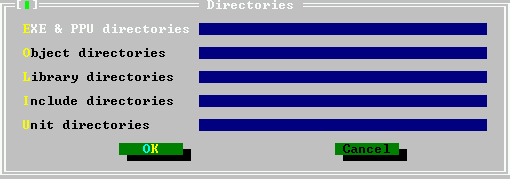
\epsfig{file=pics/ide/odirs.png,width=\textwidth}
\else
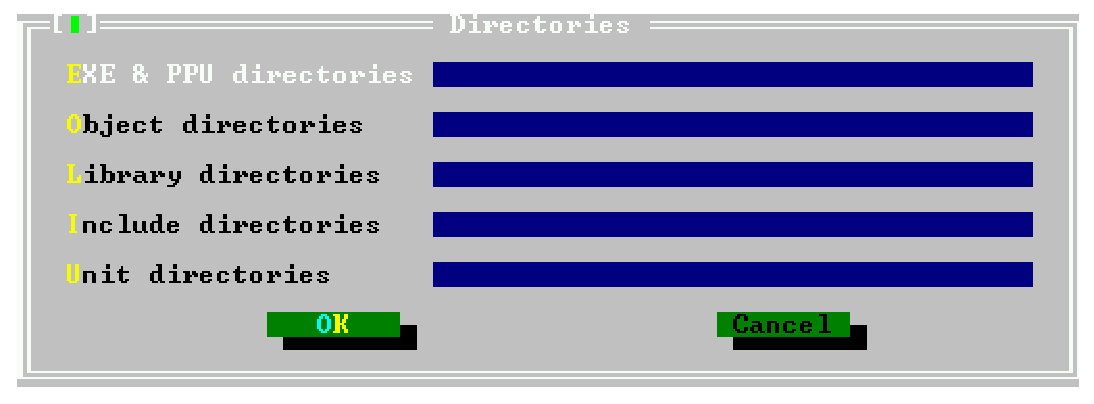
\epsfig{file=pics/ide/odirs.eps,width=\textwidth}
\fi
\end{center}
\end{figure}
\end{latexonly}
The following directories can be specified:
\begin{description}
\item[EXE \& PPU directories] Specifies where the compiled units and
executables will go. (\seeo{FE} on the command line.)
\item[Object directories] Specifies where the compiler looks for external
object files. (\seeo{Fo} on the command line.)
\item[Library directories] Specifies where the compiler (more exactly, the
linker) looks for external libraries. (\seeo{Fl} on the command line.)
\item[Include directories] Specifies where the compiler will look for 
include files, included with the \var{\{\$i \}} directive. 
(\seeo{Fi} or \seeo{I} on the command line.)
\item[Unit directories] Specifies where the compiler will look for compiled
units. The compiler always looks first in the current directory, and also in
some standard directories. (\seeo{Fu} on the command line.)
\end{description}
%
% The target operating system.
%
\subsection{The target operating system}
The menu item \menu{Compile|Target} allows to specify the target
operating system for which the sources will be compiled. 
Changing the target doesn't affect any compiler switches or 
directories. It does affect some defines defined by the compiler.
The settings here correspond to the option \seeo{T}
on the command-line.
\begin{htmlonly}
The target dialog looks as follows:
\fpcaddimg{../pics/ide/target.png}
\end{htmlonly}
\begin{latexonly}
The compilation target dialog is shown in \seefig{target}.
\begin{figure}[ht]
\begin{center}
\caption{The compilation target dialog.}\label{fig:target}
\ifpdf
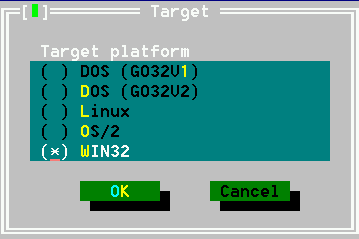
\epsfig{file=pics/ide/target.png}
\else
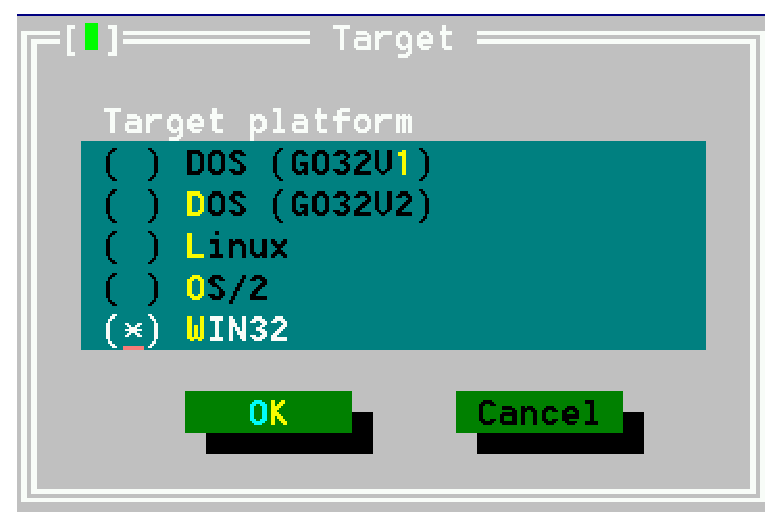
\epsfig{file=pics/ide/target.eps}
\fi
\end{center}
\end{figure}
\end{latexonly}
The following targets can be set:
\begin{description}
\item[Dos (go32v1)] This switch will dissapear in time as this target is no
longer being maintained.
\item[Dos (go32v2)] Compile for \dos, using version 2 of the Go32 extender.
\item[FreeBSD] Compile for \freebsd.
\item[Linux] Compile for \linux.
\item[OS/2] Compile for OS/2 (using the EMX extender)
\item[Win32] Compile for windows 32 bit.
\end{description}
The currently selected target operating system is shown in the menu item in
the \menu{Compile} menu. Standard this should be the operating system for
which the IDE was compiled.
%
% Other compiler options
%
\subsection{Compiler options}
The menu \menu{Options|Compiler} allows to set other options that affect the
compilers behaviour. When this menu item is chosen, a dialog pops up that
displays several tabs.

There are 5 tabs:
\begin{description}
\item[Syntax] Here options can be set that affect the various syntax aspects
of the code. They correspond mostly to the \var{-S} option on the command
line (\sees{sourceoptions}).
\item[Code generation] These options control the generated code; they are
mostly concerned with the \var{-C} and \var{-X} command-line options.
\item[Verbose] These set the verbosity of the compiler when compiling. The
messages of the compiler are shown in the compiler messages window (can be
called with \key{F12}).
\item[Browser] options concerning the generated browser information. Browser
information needs to be generated for the symbol browser to work.
\item[Assembler] Options concerning the reading of assembler blocks (-R on
the command line) and the generated assembler (\var{-A} on the command line)
\end{description}

Under the tab pages, the {\em Conditional defines} entry box is visible;
here symbols to define can be entered. The symbols should be separated with
semicolons.

\begin{htmlonly}
The syntax tab of the compiler options  looks as follows:
\fpcaddimg{../pics/ide/ocompa.png}
\end{htmlonly}
\begin{latexonly}
The syntax tab of the compiler options dialog is shown in \seefig{ocompa}.
\begin{figure}[ht]
\begin{center}
\caption{The syntax options tab.}\label{fig:ocompa}
\ifpdf
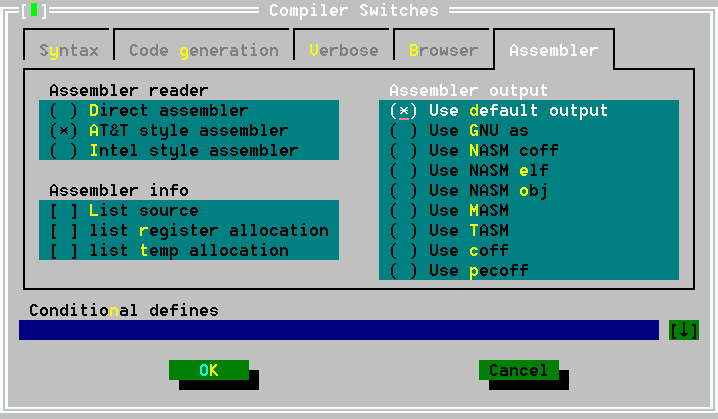
\epsfig{file=pics/ide/ocompa.png,width=\textwidth}
\else
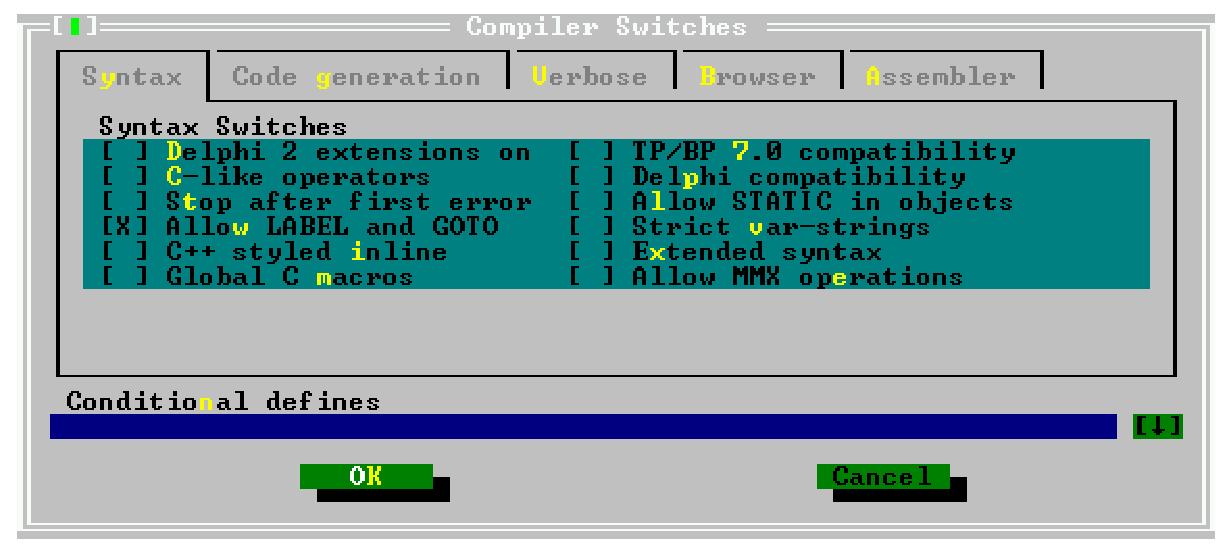
\epsfig{file=pics/ide/ocompa.eps,width=\textwidth}
\fi
\end{center}
\end{figure}
\end{latexonly}
In this dialog, the following options can be set:
\begin{description}
\item[Delphi 2 extensions on]
Enables the use of classes and exceptions (\seeo{Sd} on the command-line).
\item[C-like operators]
Allows the use of some extended operators such as \var{+=, -=} etc.
(\seeo{Sc} on the command-line).
\item[Stop after first error]  when checked, the compiler stops after the
first error. Normally the compiler continues compiling till a fatal error is
reached. (\seeo{Se} on the command-line)
\item[Allow label and goto] Allow the use of label declarations and goto
statements (\seeo{Sg} on the command line).
\item[C++ styled inline] allows the use of inlined functions (\seeo{Sc} on
the command-line).
\item[TP/BP 7.0 compatibility] Try to be more \tp compatible (\seeo{So} on
the command-line).
\item[Delphi compatibility] try to be more \delphi compatible (\seeo{Sd} on
the command-line).
\item[Allow STATIC in objects] Allow the \var{Static} modifier for object
methods (\seeo{St} on the command-line)
\item[Strict var-strings] Not used.
\item[Extended syntax] Not used.
\item[Allow MMX operations] Allow MMX operations.
\end{description}

\begin{htmlonly}
The code generation tab of the compiler options  looks as follows:
\fpcaddimg{../pics/ide/ocompb.png}
\end{htmlonly}
\begin{latexonly}
The code generation tab of the compiler options dialog is shown in
\seefig{ocompb}.
\begin{figure}[ht]
\begin{center}
\caption{The code generation options tab.}\label{fig:ocompb}
\ifpdf
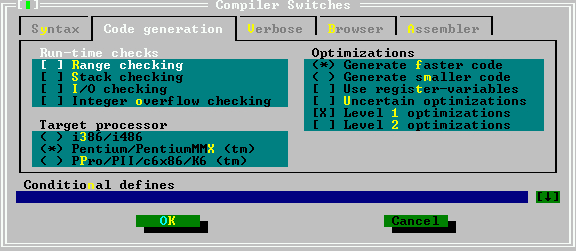
\epsfig{file=pics/ide/ocompb.png,width=\textwidth}
\else
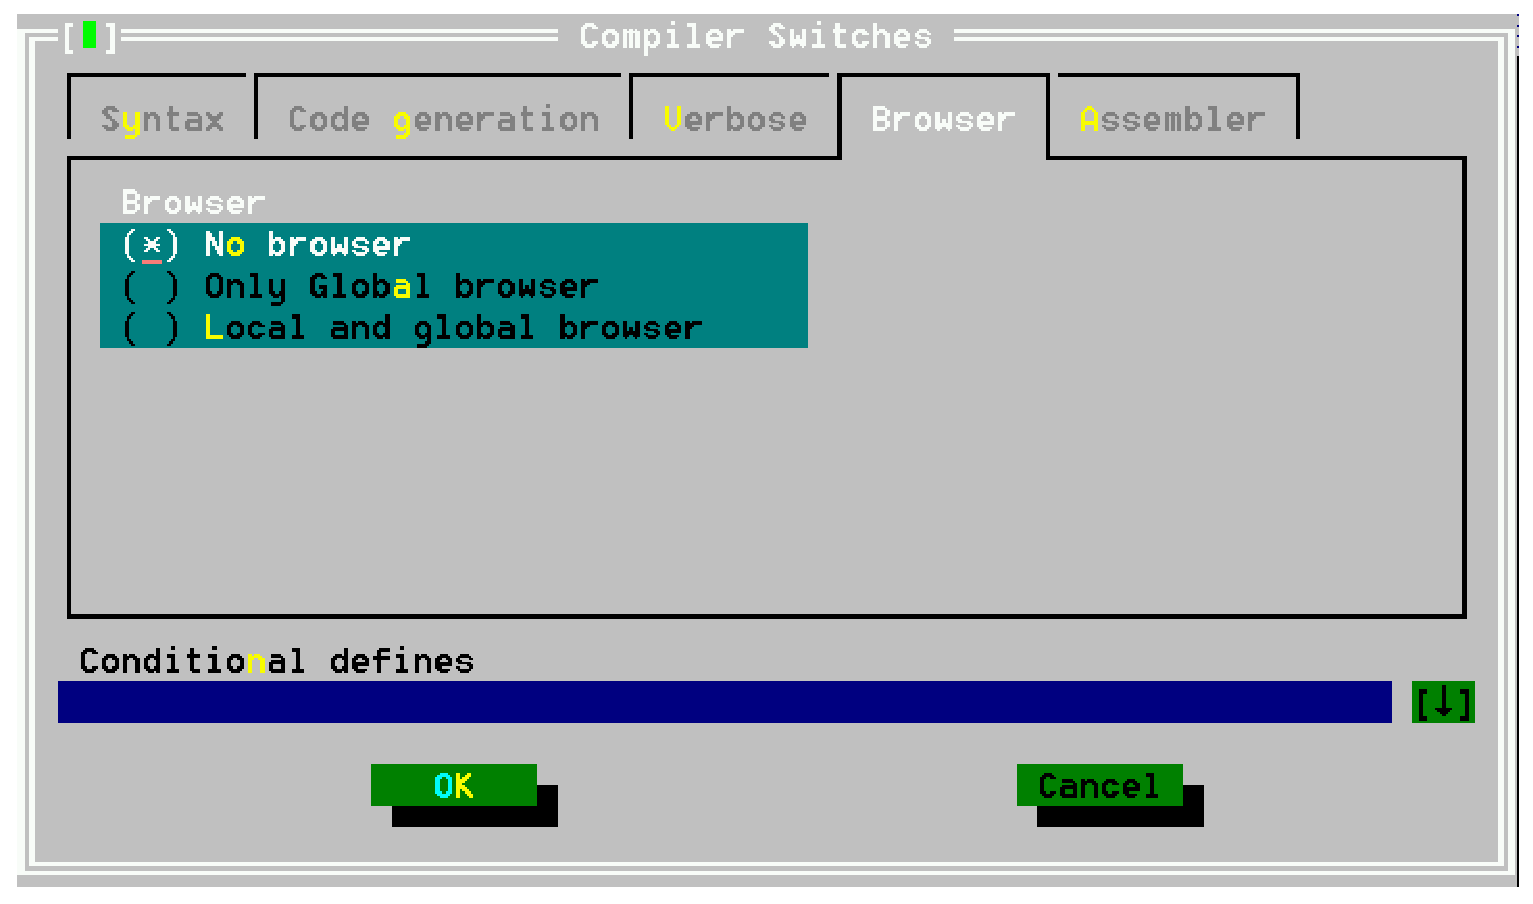
\epsfig{file=pics/ide/ocompb.eps,width=\textwidth}
\fi
\end{center}
\end{figure}
\end{latexonly}
In this dialog, the following options can be set:
\begin{description}
\item[Run-time checks] Controls what run-time checking code is generated. If
such a check fails, a run-time error is generated.
the following checking code can be generated:
\begin{description}
\item[Range checking] Code that checks the results of enumeration and subset
type operations is generated (\seeo{Cr} command-line option)
\item[Stack checking] Code that checks whether the stack limit is not
reached is generated (\seeo{Cs} command-line option)
\item[I/O checking] Code that checks the result of IO operations is
generated. (\seeo{Ci} command-line option).
\item[Integer overflow checking] The result of integer operations is
checked (\seeo{Co} command-line option)
\end{description}
\item[Target processor] Set the target process for optimizations. The
compiler can use different optimizations for different processors. This
corresponds to the \var{Op} option.
\begin{description}
\item[i386/i486] Code is optimized for less than Pentium processors.
\item[Pentium/pentiumMMX] Code is optimized for Pentium processors.
\item[PPro/PII/c6x86/K6] Code is optimized for Pentium pro and higher
processors.
\end{description}
\item[Optimizations] What optimizations should be used when compiling:
\begin{description}
\item[Generate faster code] Corresponds to the \var{-OG} command-line option.
\item[Generate smaller code] Corresponds to the \var{-Og} command-line option.
\item[Use register variables] Corresponds to the \var{-Or} command-line
option.
\item[Uncertain optimizations] Corresponds to the \var{-Ou} command-line
option.
\item[Level 1 optimizations] Corresponds to the \var{O1} command-line
option.
\item[Level 2 optimizations] Corresponds to the \var{O1} command-line
option.
\end{description}
\end{description}
More information on these switches can be found in \sees{codegen}.

\begin{htmlonly}
The verbose tab of the compiler options looks as follows:
\fpcaddimg{../pics/ide/ocompc.png}
\end{htmlonly}
\begin{latexonly}
The verbose tab of the compiler options dialog is shown in
\seefig{ocompc}.
\begin{figure}[ht]
\begin{center}
\caption{The verbosity options tab.}\label{fig:ocompc}
\ifpdf
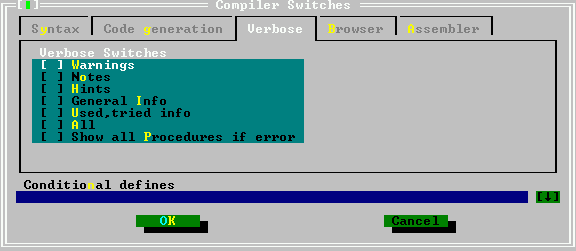
\epsfig{file=pics/ide/ocompc.png,width=\textwidth}
\else
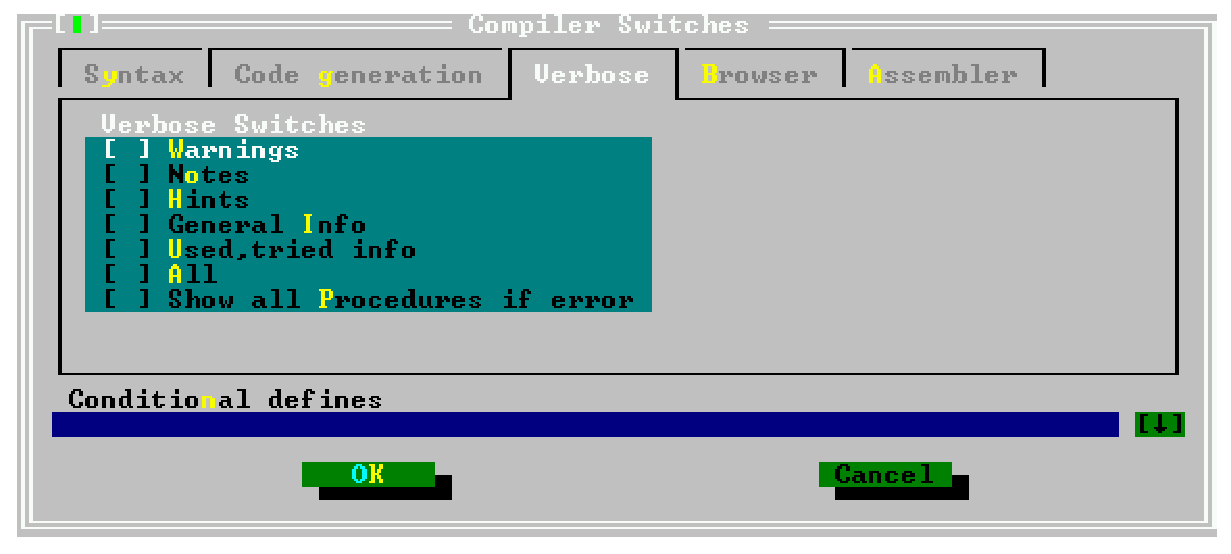
\epsfig{file=pics/ide/ocompc.eps,width=\textwidth}
\fi
\end{center}
\end{figure}
\end{latexonly}
In this dialog, the following verbosity options (\seeo{v} on the
command-line) can be set:
\begin{description}
\item[Warnings] Generate warnings, corresponds to \var{-vw} on the
command-line.
\item[Notes] Generate notes, corresponds to \var{-vn} on the
command-line.
\item[Hints] Generate hints, corresponds to \var{-vh} on the
command-line.
\item[General info] Generate general information, corresponds to \var{-vi} on the
command-line.
\item[User,tried info] Generate information on used and tried files. Corresponds to \var{-vut} on the
command-line.
\item[All] Switch on full verbosity. Corresponds to \var{-va} on the
command-line.
\item[Show all procedure if error] If an error using overloaded procedure
occurs, show all procedures. Corresponds to \var{-vb} on the
command-line.
\end{description}

\begin{htmlonly}
The browser tab of the compiler options looks as follows:
\fpcaddimg{../pics/ide/ocompd.png}
\end{htmlonly}
\begin{latexonly}
The browser tab of the compiler options dialog is shown in
\seefig{ocompd}.
\begin{figure}[ht]
\begin{center}
\caption{The browser options tab.}\label{fig:ocompd}
\ifpdf
\epsfig{file=pics/ide/ocompd.png,width=\textwidth}
\else
\epsfig{file=pics/ide/ocompd.eps,width=\textwidth}
\fi
\end{center}
\end{figure}
\end{latexonly}
In this dialog, the browser options can be set:
\begin{description}
\item[No browser] (default) no browser information is generated by the
compiler.
\item[Only global browser] Browser information is generated for global
symbols only, i.e. symbols defined not in a procedure or function (\var{-b} on the command-line)
\item[Local and global browser]  Browser information is generated for all 
symbols, i.e. also for symbols that are defined in procedures or functions 
 (\var{-bl} on the command-line)
\end{description}
\begin{remark}
If no browser information is generated, the symbol browser of the IDE will
not work.
\end{remark}

\begin{htmlonly}
The assembler tab of the compiler options looks as follows:
\fpcaddimg{../pics/ide/ocompe.png}
\end{htmlonly}
\begin{latexonly}
The assembler tab of the compiler options dialog is shown in
\seefig{ocompe}.
\begin{figure}[ht]
\begin{center}
\caption{The assembler options tab.}\label{fig:ocompe}
\ifpdf
\epsfig{file=pics/ide/ocompe.png,width=\textwidth}
\else
\epsfig{file=pics/ide/ocompe.eps,width=\textwidth}
\fi
\end{center}
\end{figure}
\end{latexonly}
In this dialog, the assembler reader and writer options can be set:
\begin{description}
\item[Assembler reader] This allows to set the style of the assembler blocks
in the sources:
\begin{description}
\item[Direct assembler] The assembler blocks are copied as-is to the output 
(\var{-Rdirect} on the command-line).
\item[AT\&T assembler] The assembler is written in \var{AT\&T} style
assembler (\var{-Ratt} on the command-line).
\item[Intel style assembler] The assembler is written in \var{Intel} style
assembler blocks (\var{-Rintel} on the command-line).
\end{description}
remark that this option is global, but locally the assembler style can be
changed with compiler directives. 
\item[Assembler info] When writing assembler files, this option decides
which extra information is written to the assembler file in comments:
\begin{description} 
\item[List source] The source lines are written to the assembler files
together with the generated assembler (\var{-al} on the command line).
\item[List register allocation] The compilers internal register
allocation/deallocation information is written to the assembler file
(\var{-ar} on the command-line).
\item[List temp allocation] The temporary register allocation/deallocation
is written to the assembler file. (\var{-at} on the command-line).
\end{description}
The latter two of these options are mainly useful for debugging the
compiler itself, it should be rarely necessary to use these.
\item[Assembler output] This option tells the compiler what assembler output
should be generated.
\begin{description}
\item[Use default output] This depends on the target.
\item[Use GNU as] assemble using \gnu \file{as} (\var{-Aas} on the
command-line).
\item[Use NASM coff] produce NASM coff assembler (go32v2, \var{-Anasmcoff} on the
command-line)
\item[Use NASM elf] produce NASM elf assembler (\linux, \var{-Anasmelf} on
the command-line).
\item[Use NASM obj] produce NASM obj assembler (\var{-Anasmobj} on the
command-line).
\item[Use MASM] produce MASM (Microsoft assembler) assembler (\var{-Amasm} on the
command-line).
\item[Use TASM] produce TASM (Turbo Assembler) assembler (\var{-Atasm} on the
command-line).
\item[Use coff] Write binary coff files directly using the internal
assembler (go32v2, \var{-Acoff} on the command-line).
\item[Use pecoff] Write binary pecoff files files directly using the
internal writer. (Win32)
\end{description}
\end{description}
%
% Linker options
%
\subsection{Linker options}
The linker options can be set in the menu \menu{Options|Linker}. It allows
to determine how libraries and units are linked, and how the linker should
be called. 
\begin{htmlonly}
The linker options dialog looks as follows:
\fpcaddimg{../pics/ide/olinker.png}
\end{htmlonly}
\begin{latexonly}
The linker options dialog is shown in
\seefig{olinker}.
\begin{figure}[ht]
\begin{center}
\caption{The linker options dialog.}\label{fig:olinker}
\ifpdf
\epsfig{file=pics/ide/olinker.png,width=\textwidth}
\else
\epsfig{file=pics/ide/olinker.eps,width=\textwidth}
\fi
\end{center}
\end{figure}
\end{latexonly}
The following options can be set:
\begin{description}
\item[Call linker after] If this option is set then a script is written
which calls the linker. This corresponds to the \seeo{s} on the
command-line.
\item[Preferred library type] With this option, the type of library to be
linked in can be set:
\begin{description}
\item[Target default] This depends on the platform.
\item[Dynamic libraries] Tries to link in units in dynamical libraries. 
(option \var{-XD} on the command-line)
\item[Static libraries] Tries to link in units in statical libraries.
(option \var{-XS} on the command-line)
\item[Smart libraries] Tries to link in units in smartlinked libraries.
(option \var{-XX} on the command-line)
\end{description}
\end{description}
%
% Memory sizes dialog
%
\subsection{Memory sizes}
The memory sizes dialog (reachable via \menu{options|Memory sizes}) allows 
to enter the memory sizes for the project.
\begin{htmlonly}
The memory sizes dialog looks as follows:
\fpcaddimg{../pics/ide/omemsize.png}
\end{htmlonly}
\begin{latexonly}
The memory sizes dialog is shown in \seefig{omemsize}.
\begin{figure}[ht]
\begin{center}
\caption{The memory sizes dialog.}\label{fig:omemsize}
\ifpdf
\epsfig{file=pics/ide/omemsize.png}
\else
\epsfig{file=pics/ide/omemsize.eps}
\fi
\end{center}
\end{figure}
\end{latexonly}
The following sizes can be entered:
\begin{description}
\item[Stack size] Sets the size of the stack in bytes; 
(option \var{-Cs} on the command line). This size may be ignored on some
systems.
\item[Heap size] Sets the size of the heap in bytes; (option \var{-Ch} on
the command-line). Note that the heap grows dynamically as much as the OS
allows.
\end{description}

%
% Debugging options
%
\subsection{Debug options}
\label{se:debugoptions}
In the debug options dialog some options for inclusion of debug information
in the binary can be set; it is also possible to add additional compiler
options in this dialog.
\begin{htmlonly}
The debug options dialog looks as follows:
\fpcaddimg{../pics/ide/odebug.png}
\end{htmlonly}
\begin{latexonly}
The debug options dialog is shown in \seefig{odebug}.
\begin{figure}[ht]
\begin{center}
\caption{The debug options dialog.}\label{fig:odebug}
\ifpdf
\epsfig{file=pics/ide/odebug.png,width=\textwidth}
\else
\epsfig{file=pics/ide/odebug.eps,width=\textwidth}
\fi
\end{center}
\end{figure}
\end{latexonly}
The following options can be set:
\begin{description}
\item[Debugging information] tells the compiler which debug information
should be compiled in. One of following options can be chosen:
\begin{description}
\item[Strip all debug symbols from executable] Will strip all debug nd
symbol information from the binary. (option \var{-Xs} on the command-line).
\item[Generate debug symbol information] include debug information in the
binary (option \var{-g} on the command-line). Please note that no debug
information for units in the Run-Time Library will be included, unless a 
version of the RTL compiled with debug information is available. Only units
specific to the current project will have debug information included.
\item[Generate also backtrace lines information] Will compile with debug
information, and will additionally include the \file{lineinfo} unit in the
binary, so in case of an error the backtrace will contain the filenames and
linenumbers of procedures in the call-stack. (Option \var{-gl} on the
command-line)
\end{description}
\item[Profiling switches] Tells the compiler whether or not profile code
should be included in the binary.
\begin{description}
\item[No profile information] Has no effect, as it is the default.
\item[Generate Profile code for gprof] If checked, profiling code is
included in the binary (option \var{-p} on the command-line).
\end{description}
\item[Addition compiler args] Here arbitrary options can be entered as they
would be entered on the command-line, they will be passed on to the compiler
as typed here.
\item[Debuggee redirection]
If checked, an attempt will be made to redirect the output of the program
being debugged to another window (terminal). 
\end{description}
 
%
% The switches mode.
%
\subsection{The switches mode}
\label{se:compilermode}
The IDE allows to save a set of compiler settings under a common name; it
provides 3 names under which the switches can be saved:
\begin{description}
\item[Normal] For normal (fast) compilation.
\item[Debug] For debugging; intended to set most debug switches on. Also
useful for setting conditional defines that e.g. allow to include some
debug code.
\item[release] For a compile of the program as it should be released, debug
information should be off, the binary should be stripped, and optimizations
should be used.
\end{description}
Selecting one of these modes will load the compiler options as they were
saved the last time the selected mode was active, i.e. it doesn't
specifically set or unset options. 

When setting and saving compiler options, be sure to select the correct
switch mode first; it makes little sense to set debug options while the
release switch is active.

\begin{htmlonly}
The switches mode dialog looks as follows:
\fpcaddimg{../pics/ide/oswitch.png}
\end{htmlonly}
\begin{latexonly}
The switches mode dialog is shown in \seefig{oswitch}.
\begin{figure}[ht]
\begin{center}
\caption{The switches mode dialog.}\label{fig:oswitch}
\ifpdf
\epsfig{file=pics/ide/oswitch.png}
\else
\epsfig{file=pics/ide/oswitch.eps}
\fi
\end{center}
\end{figure}
\end{latexonly}

%%%%%%%%%%%%%%%%%%%%%%%%%%%%%%%%%%%%%%%%%%%%%%%%%%%%%%%%%%%%%%%%%%%%%%%
% Customize the IDE
\section{Customizing the IDE}
The IDE is configurable in a wide range: Colors can be changed, screen
resolution. The configuration setting can reached via the
sub-menu \var{Environment} in the \var{Options} menu.
%
% general preferences
%
\subsection{Preferences}
The {\em preferences dialog} is called by the menu item
\menu{Options|Environment|Preferences}.
\begin{htmlonly}
The preferences dialog looks as follows:
\fpcaddimg{../pics/ide/oeprefs.png}
\end{htmlonly}
\begin{latexonly}
The preferences dialog is shown in \seefig{oprefs}.
\begin{figure}[ht]
\begin{center}
\caption{The preferences dialog.}\label{fig:oprefs}
\ifpdf
\epsfig{file=pics/ide/oeprefs.png,width=\textwidth}
\else
\epsfig{file=pics/ide/oeprefs.eps,width=\textwidth}
\fi
\end{center}
\end{figure}
\end{latexonly}
\begin{description}
\item[Video modes]
The drop down list at the top of the dialog allows to select a video mode.
The available video modes depend on the system on which the IDE
is running. 
\begin{remark}
\begin{enumerate}
\item The video mode must be selected by pressing space or clicking
on it. If the drop down list is opened while leaving the dialog,
the new video mode will not be applied.
\item For the \dos version of the IDE, the following should be noted:
When using VESA modes, the display refresh rate may be very low. 
On older graphics card (1998 and before), it is possible to use the
{\em UniVBE} driver of {\em SciTech}\footnote{It can be downloaded from
\href{http://www.informatik.fh-muenchen.de/~ifw98223/vbehz.htm}
{http://www.informatik.fh-muenchen.de/\~{}ifw98223/vbehz.htm}}
% It is quite outdated 
%(last update somewhere in 1998). 
%For newer graphics cards which support VESA 3.0, you can try to get one
%of the TSR programs
%\footnote{\textbf{T}erminate and \textbf{S}tay \textbf{R}esisdent}
% available at the net to customize the refresh rate.
%%%%!!!!!!!! footnote with URL
\end{enumerate}
\end{remark}
\item[Desktop File]
Specifies where the desktop file is saved: the current directory, or the
directory where the config file was found;
\item[Auto save]
Here it is possible to set which files are saved when a program is run or
when the IDE is exited:
\begin{description}
\item[Editor files] The contents of all open edit windows will be saved.
\item[Environment] The current environment settings will be saved
\item[Desktop] The desktop file with all desktop settings (open windows,
history lists, breakpoints etc.) will be saved.
\end{description}
\item[Options] 
Some special behaviour of the IDE can be specified here:
\begin{description}
\item[Auto track source]
\item[Close on go to source] When checked, the messages window is closed 
when the 'go to source line' action is executed.
\item[Change dir on open] When a file is opened, the directory of that file
is made the current working directory.
\end{description}
\end{description}
%
% Desktop customization
%
\subsection{The desktop}
\label{se:prefdesktop}
The desktop preferences dialog allows to specify what elements of the
desktop are saved across sessions, i.e. they are saved when the IDE is left,
and they are again restored when the IDE is started the next time. 
They are saved in a file \file{fp.dsk}.

\begin{htmlonly}
The desktop preferences dialog looks as follows:
\fpcaddimg{../pics/ide/oeprefs.png}
\end{htmlonly}
\begin{latexonly}
The desktop preferences dialog is shown in \seefig{odesktop}.
\begin{figure}[ht]
\begin{center}
\caption{The desktop preferences dialog.}\label{fig:odesktop}
\ifpdf
\epsfig{file=pics/ide/oedesk.png}
\else
\epsfig{file=pics/ide/oedesk.eps}
\fi
\end{center}
\end{figure}
\end{latexonly}
The following elements can be saved and restored across IDE sessions:
\begin{description}
\item[History lists] Most entry boxes have a history list where previous
entries are saved and can be selected. When this option is saved, these
entries are saved in the desktop file. On by default.
\item[Clipboard content]
When checked, the contents of the clipboard is also saved to disk. Off by
default.
\item[Watch expressions]
When checked, all watch expressions are saved in the desktop file. Off by
default.
\item[Breakpoints] 
When checked, all break points with their properties are saved in the
desktop file. Off by default.
\item[Open windows]
When checked, the list of files in open editor windows is saved in the 
desktop file, and the windows will be restored the next time the IDE 
is run. On by default.
\item[Symbol information]
When checked, the information for the symbol browser is saved in the desktop
file. Off by default.
\item[CodeComplete wordlist]
When checked, the list of code-completion words is saved. On by default.
\item[CodeTemplates]
When checked, the defined code-templates are saved. On by default.
\end{description}

%
% Editor customization
%
\subsection{The Editor}
Several aspects of the editor window behaviour can be set in this dialog.

\begin{htmlonly}
The editor preferences dialog looks as follows:
\fpcaddimg{../pics/ide/oeeditor.png}
\end{htmlonly}
\begin{latexonly}
The editor preferences dialog is shown in \seefig{oeeditor}.
\begin{figure}[ht]
\begin{center}
\caption{The editor preferences dialog.}\label{fig:oeeditor}
\ifpdf
\epsfig{file=pics/ide/oeeditor.png,width=\textwidth}
\else
\epsfig{file=pics/ide/oeeditor.eps,width=\textwidth}
\fi
\end{center}
\end{figure}
\end{latexonly}
The following elements can be set in the editor preferences dialog:
\begin{description}
\item[Create backup files]
Whenever an editor file is saved, a backup is made of the old file. On by
default.
\item[Auto indent mode] 
Smart indenting is on. This means that pressing \key{Enter} will position the 
cursor on the next line in the same column where text starts on the current
line. On by default.
\item[Use tab characters] 
When the tab key is pressed, use a tab character. Normally, when the tab key
is pressed, spaces are inserted. When this option is checked, tab characters 
will be inserted instead. Off by default.
\item[Backspace unindents]
Pressing the \key{Bksp} key will unindent if the beginning of the text on
the current line is reached, instead of deleting just the previous
character. On by default.
\item[Persistent blocks]
When a selection is made, and the cursor is moved, the selection is not
destroyed, i.e. the selected block stays selected. On by default. 
\item[Syntax highlight]
Use syntax highlighting on the files that have an extension which appears in
the list of highlight extensions. On by default.
\item[Block insert cursor]
The insert cursor is a block instead of an underscore character. By default
the overwrite cursor is a block. This option reverses that behaviour. Off by
default.
\item[Vertical blocks]
When selecting blocks over several lines, the block doesn't select the whole
lines in the block, it selects the lines till the column on which the cursor
is located. Off by default.
\item[Highlight column]
When checked, the current column (i.e. the column where the cursor is) is
highlighted. Off by default.
\item[Highlight row]
When checked, the current row (i.e. the row where the cursor is) is
highlighted. Off by default.
\item[Auto closing brackets]
When an opening bracket character is typed, the closing bracket is also
inserted at once. Off by default.
\item[Keep trailing spaces]
When saving a file, the spaces at the end of lines are stripped off. This
behaviour disables that behaviour, i.e. any trailing spaces are also saved
to file. Off by default.
\item[Codecomplete enabled]
Enable code completion. On by default.
\item[enable folds]
???. Off by default.
\item[Tab size]
The number of spaces that are inserted when the \key{Tab} key is pressed.
The default value is 8.
\item[Indent size]
The number of spaces a block is indented when calling the block indent function.
The default value is 2.
\item[Highlight extensions]
When syntax highlighting is on, the list of file masks entered here will be
used to determine which files are highlighted. File masks should be
separated with semicolon (;) characters. The default is
\file{*.pas;*.pp;*.inc}.
\item[File patterns needing tabs]
Some files (such as makefiles) need actual tab characters instead of spaces. 
Here a series of file masks can be entered for which tab characters will
always be used. Default is \file{make*;make*.*}.
\end{description}
\begin{remark}
These options will not be applied to already opened windows, only newly
opened windows will have these options.
\end{remark}
%
% Mouse customization
%
\subsection{Mouse}
\label{se:prefmouse}
The mouse options dialog is called by the menu item
\menu{Options|Environment|Mouse}. It allows to adjust the behaviour of the
mouse as well as the sensitivity of the mouse.
\begin{htmlonly}
The mouse options dialog looks as follows:
\fpcaddimg{../pics/ide/oemouse.png}
\end{htmlonly}
\begin{latexonly}
The mouse options dialog is shown in \seefig{omouse}.
\begin{figure}[ht]
\begin{center}
\caption{The mouse options dialog.}\label{fig:omouse}
\ifpdf
\epsfig{file=pics/ide/oemouse.png,width=\textwidth}
\else
\epsfig{file=pics/ide/oemouse.eps,width=\textwidth}
\fi
\end{center}
\end{figure}
\end{latexonly}
\begin{description}
\item[Mouse double click]
The slider can be used to adjust the double click speed. Fast means that the
time between two clicks is very short, slow means that the time between two
mouse clicks can be quite long.
\item[Reverse mouse buttons]
the behaviour of the left and right mouse buttons can be changed by
by checking the checkbox; this is especially useful for left-handed people.
\item[Ctrl+Right mouse button]
Assigns an action to a right mouse button click while holding the 
\key{Ctrl} key pressed.
\item[Ctrl+Left mouse button]
Assigns an action to a left mouse button click while holding the 
\key{Ctrl} key pressed.
\end{description}

The following actions can be assigned to \key{Ctrl}-right mouse button or
\key{Alt}-right mouse button:
\begin{description}
\item [Topic search] The keyword at the mouse cursor is searched in the
help index.
\item [Go to cursor] The program is executed until the line where
the mouse cursor is located.
\item [Breakpoint] Set a breakpoint at the mouse cursor position.
\item [Evaluate] Evaluate the value of the variable at the mouse
cursor.
\item [Add watch] Add the variable at the mouse cursor to the
watch list.
\item [Browse symbol] The symbol at the mouse cursor is displayed
in the browser.
\end{description}

%
% Color customization
%
\subsection{Colors}
\label{se:prefcolors}
Almost all elements of the IDE such as borders input fields, buttons and so
on can have their color set in this dialog. The dialog sets the colors for
all elements at once, i.e. it is not so that the color of one particular
button can be set.

The syntax highlighting colors for the editor windows of the IDE can also 
be set in this dialog.
\begin{htmlonly}
The colors dialog looks as follows:
\fpcaddimg{../pics/ide/oecolors.png}
\end{htmlonly}
\begin{latexonly}
The colors dialog is shown in \seefig{ocolors}.
\begin{figure}[ht]
\begin{center}
\caption{The colors dialog.}\label{fig:ocolors}
\ifpdf
\epsfig{file=pics/ide/oecolors.png,width=\textwidth}
\else
\epsfig{file=pics/ide/oecolors.eps,width=\textwidth}
\fi
\end{center}
\end{figure}
\end{latexonly}
The following elements are visible in the color dialog:
\begin{description}
\item[Group]
Here the group to be customized is displayed; A group is a specific window
or series of windows in the editor. A special group is {\em Syntax} which
sets the colors for syntax highlighting.
\begin{description}
\item[Browser] Sets the colors for the symbol browser window.
\item[Clock] Sets the colors for the clock in the menu.
\item[Desktop] Sets the colors for the desktop.
\item[Dialogs] Sets the colors for the dialog windows.
\item[Editor] Sets the colors for the editor windows.
\item[Help] Sets the colors for the help windows.
\item[Menus] Sets the colors used in the menus.
\item[Syntax] Sets the colors used when performing syntax highlighting in the
editor windows.
\end{description}
\item[item]
Here the item for the current group can be selected. The foreground and
background of this item can be set using the color selectors on the right of
the dialog.
\item[Foreground]
Sets the foreground color of the selected item. 
\item[background]
Sets the background color of the selected item.
\item[Sample text]
This shows the colors of the selected item in a sample text.
\end{description}
Setting a good color scheme is important especially for syntax highlighting;
a good syntax highlighting scheme helps in eliminating errors when typing,
without needing to compile the sources. 

%%%%%%%%%%%%%%%%%%%%%%%%%%%%%%%%%%%%%%%%%%%%%%%%%%%%%%%%%%%%%%%%%%%%%%%
% The help system
\section{The help system}

More information on how to handle the IDE, or about the use of various
calls in the RTL, explanations regarding the syntax of a Pascal statement,
can be found in the \emph{help system}. The help system is activated
by pressing \key{F1}.

\subsection{Navigating in the help system}
The help system contains hyperlinks; these are sensitive locations that
lead to another topic in the help system. They are marked by a different
color. The hyperlinks can be activated in 2 ways:
\begin{enumerate}
\item by clicking them with the mouse,
\item by using the \key{Tab} and \key{Shift-Tab} keys to move between 
the different hyperlinks of a page and the \key{Enter} key can be used 
to activate them.
\end{enumerate}

The contents of the help system is displayed, if \key{Shift-F1} is
pressed. To go back to the previous help topic, press \key{Alt-F1}. 
This also works if the help window isn't displayed on the desktop; the help
window will then be activated.

%
% Working with help files.
%
\subsection{Working with help files}
The IDE contains a help system which can display the following file formats:
\begin{description}
\item[TPH] The help format for the Turbo Pascal help viewer.
\item[INF] The OS/2 help format.
\item[NG] The Norton Guide Help format.
\item[HTML] HTML files. 
\end{description}
In future some more formats may be added. However, the above formats should 
cover already a wide spectrum of help files available.

\begin{remark}
Concerning the support for HTML files the following should be noted:
\begin{enumerate}
\item
The HTML viewer of the  help system is limited, it can only handle the 
most basic HTML files (graphics excluded), since it is only designed 
to display the \fpc help files. \footnote{...but feel free to improve it and send patches to the 
\fpc development team...}.
\item
When the HTML help viewer encounters a graphics file, it will try and find a
file with the same name but an extension of \file{.ans}; If this file is
found, this will be interpreted as a file with ANSI escape sequences, and 
these will be used to display a text image. The displays of the IDE dialogs
in the IDE help files are made in this way.
\end{enumerate}
\end{remark}

The menu item \menu{Help|Files} permits to add and delete help files to the
list of files in the help table of contents.
\begin{htmlonly}
The Help files dialog looks as follows:
\fpcaddimg{../pics/ide/helpfils.png}
\end{htmlonly}
\begin{latexonly}
The help files dialog is displayed in \seefig{helpfiles}.
\begin{figure}[ht]
\begin{center}
\caption{The help files dialog.}\label{fig:helpfiles}
\ifpdf
\epsfig{file=pics/ide/helpfils.png}
\else
\epsfig{file=pics/ide/helpfils.eps}
\fi
\end{center}
\end{figure}
\end{latexonly}
The dialogs lists the files that will be presented in the table of contents
window of the help system. Each entry has a small descriptive title and a
filename next to it. The following actions are available when adding help
files:
\begin{description}
\item[New] Adds a new file. IDE will display a prompt, in which the 
location of the help file should be entered. 

If the added file is an HTML file, a dialog box will be displayed
which asks for a title. This title will then be included in the
contents of help.
\item[Delete] Deletes the currently highlighted file from the help system.
It is \emph{not} deleted from the hard disk, only the help system entry is
removed.
\item[Cancel] Discards all changes and closes the dialog.
\item[OK] Saves the changes and closes the dialog.
\end{description}

The \fpc documentation in HTML format can be added to the IDE's help system,
this way the documentation can be viewed from within the IDE. If \fpc has
been installed using the installer, the installer should have added the 
FPC documentation to the list of help files, if the documentation was
installed as well.

%
% The about dialog.
%
\subsection{The about dialog}
\label{se:about}
The {\em about dialog}, reachable through (\menu{Help|About...}) shows some 
information about the IDE, such as the version number, the date it was built,
what compiler and debugger it uses. When reporting bugs about the IDE, please 
use the information given by this dialog to identify the version of the IDE
that was used.

It also displays some copyright information.

%%%%%%%%%%%%%%%%%%%%%%%%%%%%%%%%%%%%%%%%%%%%%%%%%%%%%%%%%%%%%%%%%%%%%%%
% Keyboard shortcuts
\section{Keyboard shortcuts}
\label{se:keyshortcuts}
A lot of keyboard shortcuts used by the IDE are compatible with 
WordStar and should be well known to Turbo Pascal users.

Below are the following tables:
\begin{enumerate}
\item In \seet{shortcutsgeneral} some shortcuts for handling the IDE windows
and Help are listed.
\item In \seet{shortcutscompiler} the shortcuts for compiling, running and
debugging a program are presented.
\item In \seet{shortcutsnavigation} the navigation keys are described.
\item In \seet{shortcutsedit} the editing keys are listed.
\item In \seet{shortcutsblock} lists all block command shortcuts.
\item In \seet{shortcutsselection} all selection-changing shortcuts are 
presented.
\item In \seet{shortcutsmisc} some general shortcuts are presented, 
which do not fit in the previous categories.
\end{enumerate}

\begin{FPCltable}{p{5cm}ll}{General}{shortcutsgeneral}
Command & Key shortcut & Alternative \\ \hline
Help & \key{F1} & \\
Goto last help topic & \key{Alt-F1} & \\
Search word at cursor position in help & \key{Ctrl-F1} & \\
Help index & \key{Shift-F1} & \\
Close active window & \key{Alt-F3} & \\
Zoom/Unzoom window & \key{F5} & \\
Move/Zoom active window & \key{Ctrl-F5} & \\
Switch to next window & \key{F6} & \\
Switch to last window & \key{Shift-F6} & \\
Menu & \key{F10} & \\
Local menu & \key{Alt-F10} & \\
List of windows & \key{Alt-0} & \\
Active another window & \key{Alt-<digit>} & \\
Call \file{grep} utility & \key{Shift-F2} & \\
Exit IDE & \key{Alt-X} & \\
\end{FPCltable}

%%%%%%%%%%%%%%%%%%%%%%%%%%%%%%%%%%%%%%%%%%%%%%%%%%%%%%%%%%%%%%%%%%%%%%%%%%%%
\begin{FPCltable}{p{5cm}ll}{Compiler}{shortcutscompiler}
Command & Key shortcut & Alternative \\
\hline
Reset debugger/program & \key{Ctrl-F2} & \\
Display call stack & \key{Ctrl-F3} & \\
Run til cursor & \key{F4} & \\
Switch to user screen & \key{Alt-F5} & \\
Trace into & \key{F7} & \\
Add watch & \key{Ctrl-F7} & \\
Step over & \key{F8} & \\
Set breakpoint at current line & \key{Ctrl-F8} & \\
Make & \key{F9} & \\
Run & \key{Ctrl-F9} & \\
Compile the active source file & \key{Alt-F9} & \\
Message & \key{F11} & \\
Compiler messages & \key{F12} & \\
\end{FPCltable}

%%%%%%%%%%%%%%%%%%%%%%%%%%%%%%%%%%%%%%%%%%%%%%%%%%%%%%%%%%%%%%%%%%%%%%%%%%%%
\begin{FPCltable}{p{5cm}ll}{Text navigation}{shortcutsnavigation}
Command & Key shortcut & Alternative \\
\hline
Char left & \key{Arrow left} & \key{Ctrl-S} \\
Char right & \key{Arrow right} & \key{Ctrl-D} \\
Line up & \key{Arrow up} & \key{Ctrl-E} \\
Line down & \key{Arrow down} & \key{Ctrl-X} \\
Word left & \key{Ctrl-Arrow left} & \key{Ctrl-A} \\
Word right & \key{Ctrl-Arrow right} & \key{Ctrl-F} \\
Scroll one line up & \key{Ctrl-W} & \\
Scroll one line down & \key{Ctrl-Z} & \\
Page up & \key{PageUp} & \key{Ctrl-R} \\
Page down & \key{PageDown} & \\
Beginning of Line & \key{Pos1} & \key{Ctrl-Q-S} \\
End of Line & \key{End} & \key{Ctrl-Q-D} \\
First line of window & \key{Ctrl-Pos1} & \key{Ctrl-Q-E} \\
Last line of window & \key{Ctrl-End} & \key{Ctrl-Q-X} \\
First line of file & \key{Ctrl-PageUp} & \key{Ctrl-Q-R} \\
Last line of file & \key{Ctrl-PageDown} & \key{Ctrl-Q-C} \\
Last cursor position & \key{Ctrl-Q-P} & \\
\end{FPCltable}
%%%%%%%%%%%%%%%%%%%%%%%%%%%%%%%%%%%%%%%%%%%%%%%%%%%%%%%%%%%%%%%%%%%%%%%%%%%%
\begin{FPCltable}{p{5cm}ll}{Edit}{shortcutsedit}
Command & Key shortcut & Alternative \\
\hline
Delete char & \key{Del} & \key{Ctrl-G} \\
Delete left char & \key{Backspace} & \key{Ctrl-H} \\
Delete line & \key{Ctrl-Y} & \\
Delete til end of line & \key{Ctrl-Q-Y} & \\
Delete word & \key{Ctrl-T} & \\
Insert line & \key{Ctrl-N} & \\
Toggle insert mode & \key{Insert} & \key{Ctrl-V} \\
\end{FPCltable}

%%%%%%%%%%%%%%%%%%%%%%%%%%%%%%%%%%%%%%%%%%%%%%%%%%%%%%%%%%%%%%%%%%%%%%%%%%%%
\begin{FPCltable}{p{5cm}ll}{Block commands}{shortcutsblock}
Command & Key shortcut & Alternative \\
\hline
Goto Beginning of selected text & \key{Ctrl-Q-B} & \\
Goto end of selected text & \key{Ctrl-Q-K} & \\
Select current line & \key{Ctrl-K-L} & \\
Print selected text & \key{Ctrl-K-P} & \\
Select current word & \key{Ctrl-K-T} & \\
Delete selected text & \key{Ctrl-Del} & \key{Ctrl-K-Y} \\
Copy selected text to cursor position & \key{Ctrl-K-C} & \\
Move selected text to cursor position & \key{Ctrl-K-V} & \\
Copy selected text to clipboard & \key{Ctrl-Ins} & \\
Move selected text to the clipboard & \key{Shift-Del} & \\
Indent block one column & \key{Ctrl-K-I} & \\
Unindent block one column & \key{Ctrl-K-U} & \\
Insert text from clipboard & \key{Shift-Insert} & \\
Insert file & \key{Ctrl-K-R} & \\
Write selected text to file & \key{Ctrl-K-W} & \\
Uppercase current block & \key{Ctrl-K-N} & \\
\end{FPCltable}

%%%%%%%%%%%%%%%%%%%%%%%%%%%%%%%%%%%%%%%%%%%%%%%%%%%%%%%%%%%%%%%%%%%%%%%%%%%%
\begin{FPCltable}{p{5cm}ll}{Change selection}{shortcutsselection}
Command & Key shortcut & Alternative \\
\hline
Mark beginning of selected text & \key{Ctrl-K-B} & \\
Mark end of selected text& \key{Ctrl-K-K} & \\
Remove selection & \key{Ctrl-K-Y} & \\
Extend selection one char to the left & \key{Shift-Arrow left} & \\
Extend selection one char to the right & \key{Shift-Arrow right} & \\
Extend selection to the beginning of the line & \key{Shift-Pos1} & \\
Extend selection to the end of the line & \key{Shift-End} & \\
Extend selection to the same column in the last row & \key{Shift-Arrow up} & \\
Extend selection to the same column in the next row & \key{Shift-Arrow down} & \\
Extend selection to the end of the line & \key{Shift-End} & \\
Extend selection one word to the left & \key{Ctrl-Shift-Arrow left} & \\
Extend selection one word to the right & \key{Ctrl-Shift-Arrow right} & \\
Extend selection one page up & \key{Shift-PageUp} & \\
Extend selection one page down & \key{Shift-PageDown} & \\
Extend selection to the beginning of the file & \key{Ctrl-Shift-Pos1} &
\key{Ctrl-Shift-PageUp} \\
Extend selection to the end of the file & \key{Ctrl-Shift-End} &
\key{Ctrl-Shift-PageUp} \\
\end{FPCltable}

%%%%%%%%%%%%%%%%%%%%%%%%%%%%%%%%%%%%%%%%%%%%%%%%%%%%%%%%%%%%%%%%%%%%%%%%%%%%
\begin{FPCltable}{p{5cm}ll}{Misc. commands}{shortcutsmisc}
Command & Key shortcut & Alternative \\
\hline
Save file & \key{F2} & \key{Ctrl-K-S} \\
Open file & \key{F3} & \\
Search & \key{Ctrl-Q-F} & \\
Search again & \key{Ctrl-L}\ & \\
Search and replace & \key{Ctrl-Q-A} & \\
Set mark & \key{Ctrl-K-n} (where n can be 0..9) & \\
Goto mark & \key{Ctrl-Q-n} (where n can be 0..9) & \\
Undo & \key{Alt-Backspace} & \\
\end{FPCltable}
%
%  $Log$
%  Revision 1.4  2001-11-05 19:08:47  michael
%  + Some small corrections before 1.0.6
%
%  Revision 1.3  2001/07/19 15:07:56  michael
%  + Merged from fixbranch
%
%  Revision 1.1.2.21  2001/06/29 19:44:47  peter
%    * create pdf without latex2html installed
%
%  Revision 1.1.2.20  2000/12/08 23:59:53  michael
%  + Some changes noted by marco
%
%  Revision 1.1.2.19  2000/12/08 21:15:39  michael
%  + spell-checked
%
%  Revision 1.1.2.18  2000/12/08 20:41:50  michael
%  + Fixed some references
%
%  Revision 1.1.2.17  2000/12/08 16:55:54  michael
%  + Some remarks corrected
%
%  Revision 1.1.2.16  2000/12/08 12:57:21  michael
%  + Documented tdf format
%
%  Revision 1.1.2.15  2000/12/07 23:19:04  michael
%  + Added memsizes, goto line and debug options
%
%  Revision 1.1.2.14  2000/12/06 23:08:56  michael
%  + Linker options dialog documented
%
%  Revision 1.1.2.13  2000/12/03 22:32:06  michael
%  + More compiler options
%
%  Revision 1.1.2.12  2000/11/28 22:53:06  michael
%  + Better sized pictures, start of options
%
%  Revision 1.1.2.11  2000/11/21 22:02:25  peter
%    * html image including fixed
%
%  Revision 1.1.2.10  2000/11/21 18:44:38  peter
%    * removed last gifs
%
%  Revision 1.1.2.9  2000/11/21 14:16:06  michael
%  + Pages 1-23 corrected after remarks from Luk Vandelaer
%
%  Revision 1.1.2.8  2000/11/20 18:53:52  michael
%  + Documenting tools
%
%  Revision 1.1.2.7  2000/11/19 23:08:32  michael
%  + Further implementation.
%
%  Revision 1.1.2.6  2000/11/18 00:06:11  michael
%  + Added code templates
%  + Added syntax highlighting
%  + Added codecompletion
%  + Added gdb window
%
%  Revision 1.1.2.5  2000/11/15 23:43:32  michael
%  + Debugging finished
%
%  Revision 1.1.2.4  2000/11/15 18:58:35  michael
%  + Debug continued
%
%  Revision 1.1.2.3  2000/11/14 23:24:09  michael
%  + Documented run menu
%
%  Revision 1.1.2.2  2000/11/13 23:46:03  michael
%  + documented blocks, search, and the browser
%
%  Revision 1.1.2.1  2000/11/12 23:40:32  michael
%  + Changes for final version
%
%  Revision 1.1  2000/07/13 09:10:04  michael
%  + Initial import
%
%  Revision 1.5  2000/03/04 07:47:28  florian
%    * some corrections and some new stuff
%
%  Revision 1.4  2000/03/01 15:39:40  florian
%    * some new stuff
%
%  Revision 1.3  2000/02/28 17:45:40  florian
%    * a lot of new stuff
%
